% !TeX root = srs.tex
% !TeX program = pdflatex
\documentclass[11pt,a4paper]{article}

% Allow inclusion of PDF figures exported with newer PDF versions
\pdfminorversion=7

% =====================
% Packages
% =====================
\usepackage[top=0.9in,left=0.9in,right=0.9in,bottom=1.2in]{geometry}
\usepackage{array}
\usepackage{ragged2e}
\usepackage{setspace}
\usepackage{hyperref}
\usepackage{enumitem}
\usepackage{graphicx}
\usepackage{eso-pic}  % Background images
\usepackage{fancyhdr}
\usepackage{tabularx}
\usepackage{booktabs}
\usepackage{multirow}
\usepackage{float}
\usepackage{xcolor}
\usepackage{parskip}
\usepackage{amsmath}
\usepackage{amssymb}
\usepackage{colortbl}
\usepackage{longtable}
\usepackage{textcomp}
\usepackage{caption}
\usepackage{bookmark}
\usepackage[normalem]{ulem}
\hypersetup{
  colorlinks=true,
  linkcolor=blue,
  urlcolor=blue,
  citecolor=blue
}
% Make all hyperlinks blue AND underlined
\AtBeginDocument{%
  \let\origref\ref
  \renewcommand{\ref}[1]{\uline{\origref{#1}}}%
  \let\orighyperref\hyperref
  \renewcommand{\hyperref}[2][]{\orighyperref[#1]{\uline{#2}}}%
}
\definecolor{tableheader}{RGB}{240, 240, 240}
\definecolor{tablerow}{RGB}{250, 250, 250}
\frenchspacing

% =====================
% Font (pdflatex-friendly Arial-like)
% =====================
\usepackage[T1]{fontenc}
\usepackage[scaled=0.95]{helvet}
\renewcommand{\familydefault}{\sfdefault}

\setstretch{1.0}

% =====================
% BACKGROUND IMAGES SETUP
% =====================
% Cover page (Page 1): Brigman_Letterhead.pdf
% All other pages: Brigman_Paper.pdf
\AddToShipoutPictureBG*{%
  \AtPageLowerLeft{%
    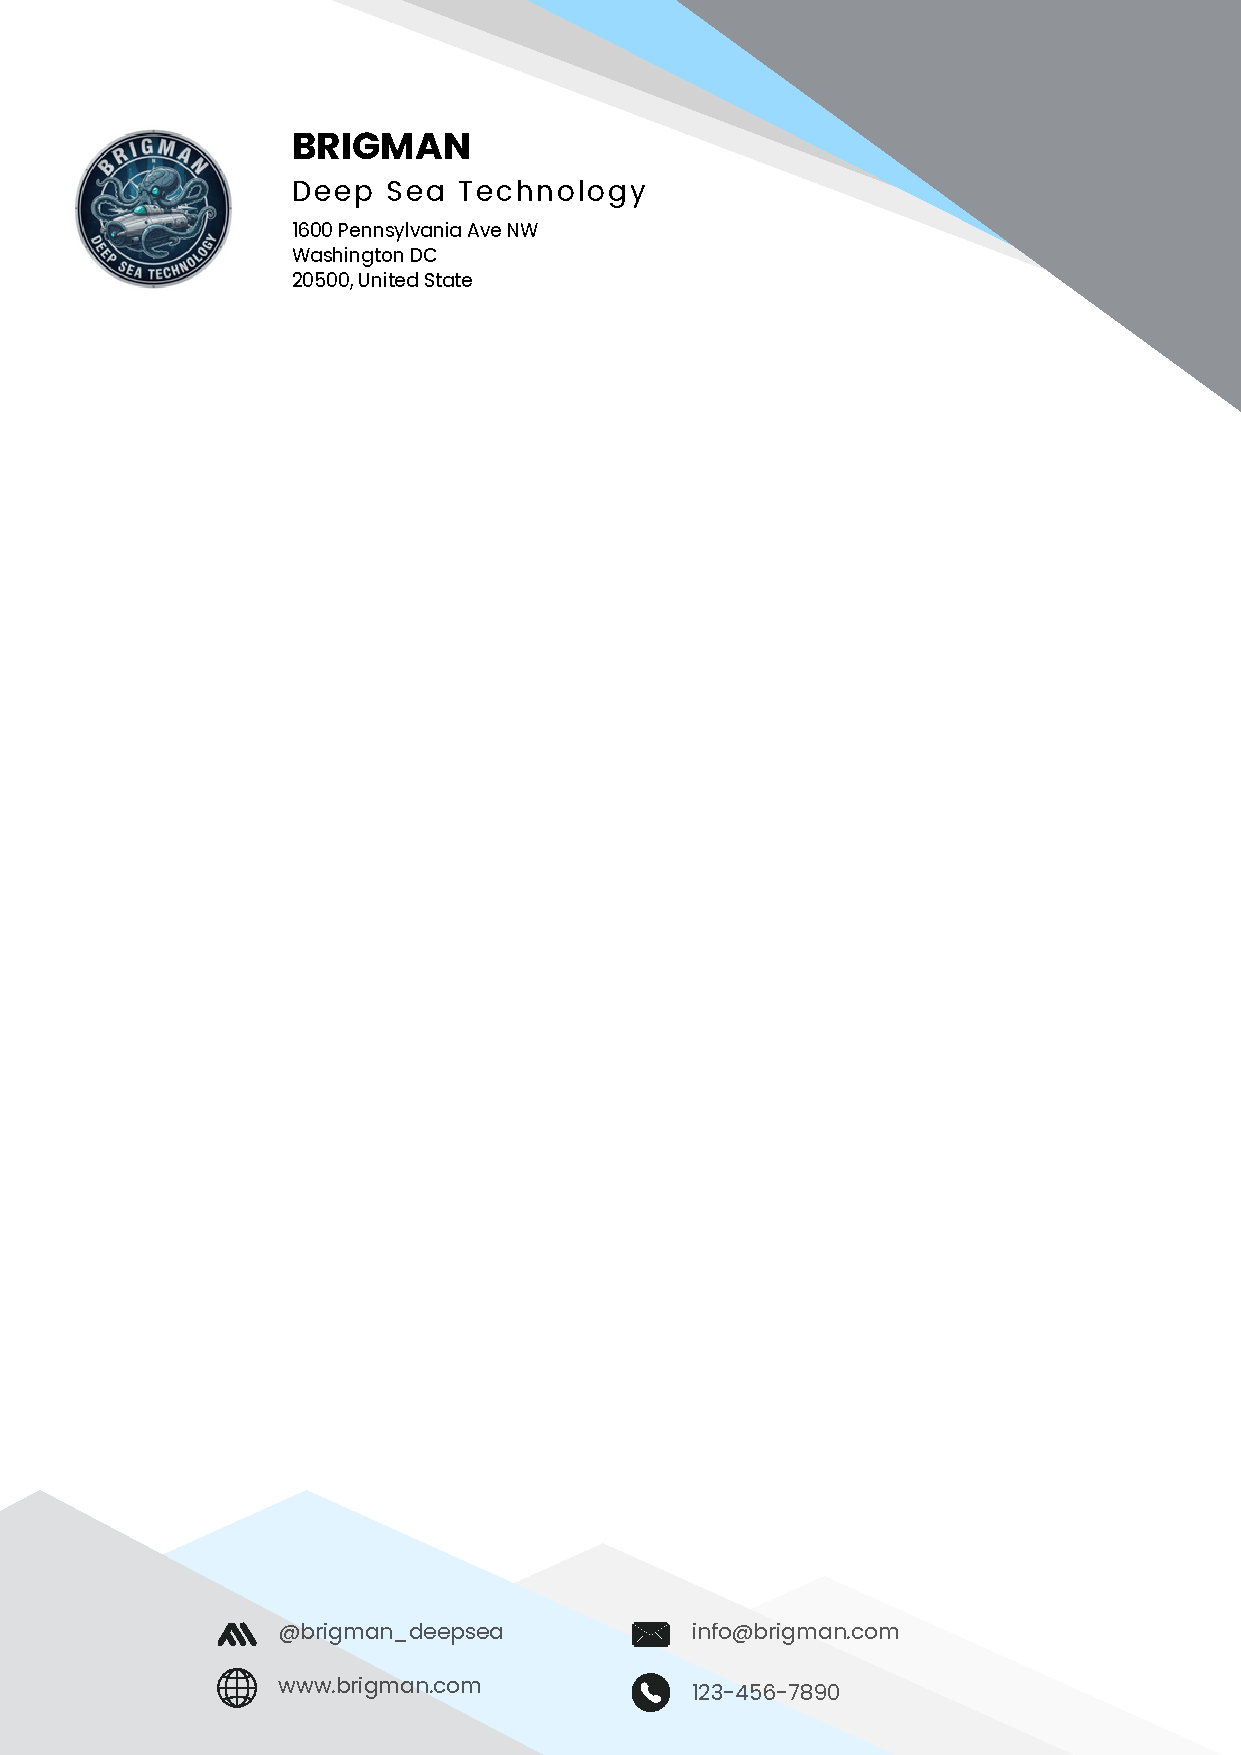
\includegraphics[width=\paperwidth,height=\paperheight]{../templates/Brigman_Letterhead.pdf}%
  }%
}
\AddToShipoutPictureBG{%
  \ifnum\value{page}>1
    \AtPageLowerLeft{%
      
\includegraphics[width=\paperwidth,height=\paperheight]{../templates/Brigman_Paper.pdf}%
    }%
  \fi
}

% =====================
% Header/Footer (page numbers must appear)
% =====================
\pagestyle{fancy}
\fancyhf{}
\lhead{\textbf{Brigman Deep Sea Technology}}
\rhead{Software Requirements Specification (SRS)}
\cfoot{\thepage}
\renewcommand{\headrulewidth}{0.4pt}
\setlength{\headheight}{20pt}

\begin{document}

% =====================
% COVER PAGE (no page number)
% =====================
\thispagestyle{empty}
\fancyhf{}
\lhead{}
\rhead{}
\cfoot{}
\renewcommand{\headrulewidth}{0pt}

\newgeometry{top=5.2cm,left=0.9in,right=0.9in,bottom=1.2in}

\begin{center}

\includegraphics[width=0.4\textwidth]{../templates/brigman logo.png}\\[0.5cm]

\LARGE\textbf{Software Requirements Specification (SRS)}\\[0.4cm]
\large\textbf{Abyss Navigator Suite Project}\\[0.6cm]

\textbf{\Large Brigman Deep Sea Technology}\\
\today
\end{center}

\begin{table}[H]
\centering
\small
\renewcommand{\arraystretch}{2.0}
\begin{tabular}{|>{\raggedright\arraybackslash}m{0.25\textwidth}|>{\raggedright\arraybackslash}m{0.2\textwidth}|>{\raggedright\arraybackslash}m{0.25\textwidth}|>{\raggedright\arraybackslash}m{0.2\textwidth}|}
\hline
\rowcolor{tableheader}
\textbf{Brigman Team Member} & \textbf{Department} & \textbf{Role} & \textbf{Employee ID} \\
\hline
Muhammad Ridwan Putra Jasni & Requirements Engineering & Lead Business Analyst & BDST-RE-BA-001 \\
\hline
Chng Zong Han & Requirements Engineering & Business Analyst & BDST-RE-BA-002 \\
\hline
Lin Yuhao & Requirements Engineering & Business Analyst & BDST-RE-BA-003 \\
\hline
Muhammad Mikhail Bin Mazlan & Requirements Engineering & Business Analyst & BDST-RE-BA-004 \\
\hline
Kannan s/o Rajamohan & Requirements Engineering & Business Analyst & BDST-RE-BA-005 \\
\hline
\end{tabular}
\caption{Requirements Engineering Team -- Brigman Deep Sea Technology}
\label{tab:re-team}
\end{table}

\restoregeometry
\newpage

% Restore standard headers for rest of document
\pagestyle{fancy}
\fancyhf{}
\lhead{\textbf{Brigman Deep Sea Technology}}
\rhead{Software Requirements Specification (SRS)}
\cfoot{\thepage}
\renewcommand{\headrulewidth}{0.4pt}
\setlength{\headheight}{20pt}

% =====================
% FRONT MATTER
% =====================
\renewcommand{\contentsname}{Table of Contents}
\thispagestyle{empty}
\hypersetup{linkcolor=black}
\tableofcontents
\newpage
\hypersetup{linkcolor=blue}

\noindent\fbox{\begin{minipage}{\dimexpr\textwidth-2\fboxsep-2\fboxrule\relax}
  \small\textbf{Note on Hyperlinks:} Throughout this document, all hyperlinks are displayed in \textcolor{blue}{\underline{blue and underlined}}. These links are fully clickable in the PDF viewer and will navigate to the relevant section, requirement, or external resource.
\end{minipage}}

\bigskip

% =====================
% 1. INTRODUCTION
% =====================
\section{Introduction}

\subsection{Purpose}
This Software Requirements Specification (SRS) defines the software requirements for the \textbf{Abyss Navigator Suite}, an unmanned deep-sea submersible fleet control system for Triton Deepwater. It is intended to be the baseline agreement for design, implementation, verification, and change control.

\subsection{Document Conventions}
\textbf{Template source.} This SRS is structured using the \textit{Software Requirements Specification} template by \textbf{Karl E. Wiegers (1999)} (provided in \texttt{References/srs\_template-ieee.pdf}), adapted to incorporate the course rubric requirements (codification, iRTM, and change mitigation).

\textbf{Normative language.} All requirements use \textbf{shall} to indicate mandatory behavior.

\textbf{Codification (mandatory).} The following ID schemes are used throughout:
\begin{itemize}[leftmargin=*,nosep]
  \item \textbf{Software requirements:} \texttt{<DOMAIN>-<FEATURE>-<NNN>} (e.g., \texttt{SAF-EMG-001}).
  \item \textbf{Technology requirements:} \texttt{TECH-<AREA>-<NNN>} (e.g., \texttt{TECH-PLAT-001}).
  \item \textbf{Quality model features:} \texttt{QUAL-<AREA>-<NNN>} (e.g., \texttt{QUAL-SAF-001}).
  \item \textbf{iRTM entries:} \texttt{RTM-<NNN>} (e.g., \texttt{RTM-001}).
  \item \textbf{Change mitigation controls:} \texttt{CHG-<AREA>-<NNN>} (e.g., \texttt{CHG-CONT-001}, \texttt{CHG-OISS-001}, \texttt{CHG-HRCC-001}).
\end{itemize}

\textbf{Priority levels.} Priority is recorded as \textbf{Essential}, \textbf{Desirable}, or \textbf{Acceptable} to align with the Project Specification.

\subsection{Intended Audience and Reading Suggestions}
This SRS is intended for Triton Deepwater stakeholders, the Brigman development and verification teams, project management, and independent auditors. Readers should begin with Sections 1--3 (scope, constraints, codification) before using Section 4 (requirements) and Sections 7--8 (traceability and change mitigation).

\subsection{Product Scope}
The Abyss Navigator Suite enables unmanned missions executed autonomously, remotely supervised from a surface or mothership environment, with controlled intervention, safe emergency handling, and operational traceability.

% =====================
% 2. OVERALL DESCRIPTION
% =====================
\section{Overall Description}

\subsection{Product Functions}
At a high level, the system provides:
\begin{itemize}[leftmargin=*,nosep]
  \item Mission planning and autonomous execution for unmanned deep-sea missions.
  \item Remote monitoring, operator alerting, and controlled remote intervention.
  \item Fleet-level supervision for multiple submersibles concurrently.
  \item Emergency detection, safe-state transition, and recovery coordination.
  \item Secure operational data management, logging, and post-mission traceability.
\end{itemize}

\subsection{User Classes and Characteristics}
\begin{itemize}[leftmargin=*,nosep]
  \item \textbf{Mission Supervisor:} monitors mission progress and authorizes intervention.
  \item \textbf{Fleet Operator:} manages multi-vehicle assignments and scheduling.
  \item \textbf{Safety \& Compliance Officer:} reviews anomalies, audits logs, and ensures governance obligations are met.
  \item \textbf{System Administrator:} manages credentials, configuration, and system health.
  \item \textbf{Data Analyst:} exports mission data for downstream analysis.
\end{itemize}

\subsection{Operating Environment (Latest Tech)}
The operating environment is characterized by remote supervision from a mothership environment and constrained connectivity to submersibles. The vendor-selected software platform is described in Section~\ref{sec:tech-reqs}. Key operating constraints include:
\begin{itemize}[leftmargin=*,nosep]
  \item Underwater communications may be intermittent and low-bandwidth.
  \item Extreme pressure and low visibility increase reliance on sensor-driven autonomy.
  \item Operational data is safety- and audit-relevant and must be protected.
\end{itemize}

\subsection{Design and Implementation Constraints}
The following constraints apply:
\begin{itemize}[leftmargin=*,nosep]
  \item \textbf{Remote operations context:} mission supervision and control are performed remotely from surface/mothership environments.
  \item \textbf{Communications constraints:} the system must operate under constrained bandwidth/latency and intermittent connectivity.
  \item \textbf{Security and governance:} operational data protection and auditability are required.
  \item \textbf{Safety-first policy:} failures and abnormal conditions must bias toward safe-state behavior.
\end{itemize}

\subsection{User Documentation}
The following documentation shall be delivered with the software:
\begin{itemize}[leftmargin=*,nosep]
  \item Operator manual (mission planning, supervision, interventions, safety procedures).
  \item System administration guide (credentials, configuration, deployment).
  \item Interface/API guide for integrating Triton-provided sensors and external systems.
\end{itemize}

\subsection{Assumptions and Dependencies}
\begin{itemize}[leftmargin=*,nosep]
  \item Triton provides mission sensors and their interface specifications for integration.
  \item Missions are supervised by trained and authorized personnel.
  \item Regulatory obligations apply to maritime safety and data governance.
\end{itemize}

% =====================
% 3. CODIFICATION
% =====================
\section{Codification}
\label{sec:codification}

\subsection{Codification Rules}
\textbf{Requirement IDs} are stable across revisions. The numeric suffix increments only when a new requirement is added; edited requirements retain their IDs to preserve traceability in the iRTM.

\subsection{Requirement Attributes and Quality Tagging}
Each requirement in Section 4 is recorded with:
\begin{itemize}[leftmargin=*,nosep]
  \item \textbf{Source:} originating Project Specification clause(s) (e.g., \texttt{BO-L1-4}, \texttt{IT-L0-C3}).
  \item \textbf{Priority:} Essential / Desirable / Acceptable.
  \item \textbf{Quality tags:} one or more \texttt{QUAL-*} IDs from Section~\ref{sec:quality-model}.
  \item \textbf{Verification:} inspection, analysis, test, or demonstration.
  \item \textbf{Use Case link:} reference to the primary use case(s) in Figure~\ref{fig:usecase-diagram-pdf} (numbered \texttt{UC01}, \texttt{UC02}, \dots) that realize or exercise the requirement.
\end{itemize}

% =====================
% 4. SPECIFIC REQUIREMENTS
% =====================
\section{Specific Requirements}
\label{sec:requirements}

\subsection{Navigation \& Mission Autonomy}
\small
\renewcommand{\arraystretch}{1.2}
\setlength{\tabcolsep}{3pt}
\begin{longtable}{|>{\raggedright\arraybackslash}p{0.12\textwidth}|>{\raggedright\arraybackslash}p{0.08\textwidth}|>{\raggedright\arraybackslash}p{0.12\textwidth}|>{\raggedright\arraybackslash}p{0.12\textwidth}|>{\raggedright\arraybackslash}p{0.29\textwidth}|>{\raggedright\arraybackslash}p{0.15\textwidth}|>{\raggedright\arraybackslash}p{0.12\textwidth}|}
\hline
\rowcolor{tableheader}
\textbf{Req ID} & \textbf{Priority} & \textbf{Source} & \textbf{Quality Tags} & \textbf{Requirement} & \textbf{Verification} & \textbf{Use Case Link} \\
\hline
\endfirsthead
\hline
\rowcolor{tableheader}
\textbf{Req ID} & \textbf{Priority} & \textbf{Source} & \textbf{Quality Tags} & \textbf{Requirement} & \textbf{Verification} & \textbf{Use Case Link} \\
\hline
\endhead
\hline \multicolumn{7}{r}{{Continued on next page}} \\ \hline
\endfoot
\hline
\endlastfoot

NAV-PLAN-001 & Essential & BO-L1-1 & QUAL-OPS-001, QUAL-TRC-001 & Upon submission by an authorized operator, the system shall create and version-control a mission plan record containing an ordered set of waypoints (latitude, longitude, depth) and mission phases, creating a new version record upon each subsequent modification. & Demo: Create/edit/version plan; inspect stored plan versions. & \hyperref[fig:usecase-diagram-pdf]{UC01} (Mission planning) \\
\hline
NAV-EXEC-001 & Essential & BO-L1-1, BO-L0-C1 & QUAL-RES-001, QUAL-SAF-001 & The system shall execute a validated mission plan autonomously without continuous human control for a full mission cycle in a representative simulation. & Test: End-to-end mission simulation with no operator commands. & \hyperref[fig:usecase-diagram-pdf]{UC02} (Autonomous mission execution) \\
\hline
NAV-WPT-001 & Essential & BO-L1-1 & QUAL-OPS-001 & The system shall achieve \textbf{99\% waypoint arrival success} in which each reached waypoint is within \(\leq\)5 m horizontal and \(\leq\)2 m vertical error under representative sea-trial conditions. & Analysis: Compare logged track vs. waypoints across trials. & \hyperref[fig:usecase-diagram-pdf]{UC02} (Waypoint navigation) \\
\hline
NAV-FLEET-001 & Desirable & BO-L1-3, IT-L1-3 & QUAL-OPS-001, QUAL-RES-001 & The system shall assign mission plans to and retrieve real-time status from at least \textbf{3} concurrently supervised submersibles within a single supervision session. & Test: Simulated 3-vehicle session; verify assignment and visibility. & \hyperref[fig:usecase-diagram-pdf]{UC03} (Supervise multiple vehicles) \\
\hline
\caption{Navigation \& Mission Autonomy Requirements}\label{tab:req-navigation}
\end{longtable}
\setlength{\tabcolsep}{6pt}
\normalsize

\subsection{Communications \& Remote Operations}
\small
\renewcommand{\arraystretch}{1.2}
\setlength{\tabcolsep}{3pt}
\begin{longtable}{|>{\raggedright\arraybackslash}p{0.12\textwidth}|>{\raggedright\arraybackslash}p{0.08\textwidth}|>{\raggedright\arraybackslash}p{0.12\textwidth}|>{\raggedright\arraybackslash}p{0.12\textwidth}|>{\raggedright\arraybackslash}p{0.29\textwidth}|>{\raggedright\arraybackslash}p{0.15\textwidth}|>{\raggedright\arraybackslash}p{0.12\textwidth}|}
\hline
\rowcolor{tableheader}
\textbf{Req ID} & \textbf{Priority} & \textbf{Source} & \textbf{Quality Tags} & \textbf{Requirement} & \textbf{Verification} & \textbf{Use Case Link} \\
\hline
\endfirsthead
\hline
\rowcolor{tableheader}
\textbf{Req ID} & \textbf{Priority} & \textbf{Source} & \textbf{Quality Tags} & \textbf{Requirement} & \textbf{Verification} & \textbf{Use Case Link} \\
\hline
\endhead
\hline \multicolumn{7}{r}{{Continued on next page}} \\ \hline
\endfoot
\hline
\endlastfoot

COM-MON-001 & Essential & BO-L1-2, IT-L1-1 & QUAL-OPS-001 & The system shall retrieve mission and vehicle status data and transmit telemetry updates to the operator interface at least once every \textbf{30 seconds} when connectivity is available. & Test: Measure telemetry update intervals under nominal link. & \hyperref[fig:usecase-diagram-pdf]{UC04} (Monitor telemetry) \\
\hline
COM-INT-001 & Essential & IT-L1-2, BO-L1-2 & QUAL-OPS-001, QUAL-SAF-001 & The system shall accept, execute, and record an acknowledgement for remote intervention commands (pause, resume, safe-state) issued by an authorized operator, delivering the acknowledgement within \(\leq\)\textbf{60 seconds} when link latency is \(\leq\)30 seconds. & Test: Command/ack timing under simulated 30s latency. & \hyperref[fig:usecase-diagram-pdf]{UC05} (Remote intervention) \\
\hline
COM-DEG-001 & Essential & IT-L0-C2, IT-L1-6 & QUAL-RES-001, QUAL-SAF-001 & The system shall support safe operation under constrained communications, including operation at \(\geq\) \textbf{1 kbps} bandwidth, \(\leq\) \textbf{30 s} one-way latency, and intermittent connectivity, and shall enter safe-state if connectivity is lost continuously for \(>\) \textbf{10 minutes}. & Test: Fault-inject bandwidth, latency, and outage; verify safe-state trigger. & \hyperref[fig:usecase-diagram-pdf]{UC06} (Handle degraded comms) \\
\hline
\caption{Communications \& Remote Operations Requirements}\label{tab:req-communications}
\end{longtable}
\setlength{\tabcolsep}{6pt}
\normalsize

\subsection{Safety \& Recovery}
\small
\renewcommand{\arraystretch}{1.2}
\setlength{\tabcolsep}{3pt}
\begin{longtable}{|>{\raggedright\arraybackslash}p{0.12\textwidth}|>{\raggedright\arraybackslash}p{0.08\textwidth}|>{\raggedright\arraybackslash}p{0.12\textwidth}|>{\raggedright\arraybackslash}p{0.12\textwidth}|>{\raggedright\arraybackslash}p{0.29\textwidth}|>{\raggedright\arraybackslash}p{0.15\textwidth}|>{\raggedright\arraybackslash}p{0.12\textwidth}|}
\hline
\rowcolor{tableheader}
\textbf{Req ID} & \textbf{Priority} & \textbf{Source} & \textbf{Quality Tags} & \textbf{Requirement} & \textbf{Verification} & \textbf{Use Case Link} \\
\hline
\endfirsthead
\hline
\rowcolor{tableheader}
\textbf{Req ID} & \textbf{Priority} & \textbf{Source} & \textbf{Quality Tags} & \textbf{Requirement} & \textbf{Verification} & \textbf{Use Case Link} \\
\hline
\endhead
\hline \multicolumn{7}{r}{{Continued on next page}} \\ \hline
\endfoot
\hline
\endlastfoot

SAF-EMG-001 & Essential & BO-L1-4, BO-L2-4.1 & QUAL-SAF-001, QUAL-OPS-001 & The system shall detect pressure deviations \(>\pm5\%\) from nominal setpoint within \textbf{5 seconds}. & Test: Inject simulated pressure spike; measure detection latency. & \hyperref[fig:usecase-diagram-pdf]{UC07} (Detect anomalies) \\
\hline
SAF-EMG-002 & Essential & BO-L1-4, BO-L2-4.1 & QUAL-SAF-001, QUAL-OPS-001 & The system shall detect temperature deviations \(>\pm10\%\) from nominal within \textbf{10 seconds}. & Test: Thermal chamber simulation or sensor-in-the-loop test. & \hyperref[fig:usecase-diagram-pdf]{UC07} (Detect anomalies) \\
\hline
SAF-EMG-003 & Essential & BO-L1-4, BO-L2-4.1 & QUAL-SAF-001, QUAL-OPS-001 & The system shall detect power supply deviations \(>\pm15\%\) from nominal within \textbf{10 seconds}. & Test: Power supply fault injection; measure detection latency. & \hyperref[fig:usecase-diagram-pdf]{UC07} (Detect anomalies) \\
\hline
SAF-STATE-001 & Essential & BO-L2-4.2 & QUAL-SAF-001 & Upon detection of any abnormal condition, the system shall transition the submersible to a \textbf{safe operational state} defined as neutral buoyancy, minimal power consumption, and active communication beacon. & Integration test: End-to-end emergency scenario. & \hyperref[fig:usecase-diagram-pdf]{UC08} (Enter safe state) \\
\hline
SYS-CONT-001 & Essential & BO-L1-5 & QUAL-RES-001, QUAL-SAF-001 & When non-critical degradation occurs, the system shall continue the mission in a degraded mode while alerting the operator and logging the degradation event. & Test: Inject non-critical fault; confirm degraded continuation and alert/log. & \hyperref[fig:usecase-diagram-pdf]{UC09} (Continue in degraded mode) \\
\hline
SYS-TERM-001 & Essential & BO-L1-5 & QUAL-SAF-001, QUAL-TRC-001 & When termination is required, the system shall terminate the mission in an orderly manner by completing the current operation when safe, logging the shutdown reason, and entering safe-state. & Test: Inject critical fault; verify ordered termination sequence. & \hyperref[fig:usecase-diagram-pdf]{UC10} (Terminate mission) \\
\hline
SYS-REC-001 & Essential & BO-L1-5 & QUAL-SAF-001, QUAL-OPS-001 & The system shall autonomously initiate emergency retrieval procedures without operator command upon entry into safe-state due to critical failure. The system shall continuously broadcast a recovery beacon and expose last-known position and status to operators until recovery is confirmed. & Demo/Test: Simulate safe-state; verify beacon and status visibility. & \hyperref[fig:usecase-diagram-pdf]{UC11} (Coordinate recovery) \\
\hline
\caption{Safety \& Recovery Requirements}\label{tab:req-safety}
\end{longtable}
\setlength{\tabcolsep}{6pt}
\normalsize

\subsection{Data Logging \& Accountability}
\small
\renewcommand{\arraystretch}{1.2}
\setlength{\tabcolsep}{3pt}
\begin{longtable}{|>{\raggedright\arraybackslash}p{0.12\textwidth}|>{\raggedright\arraybackslash}p{0.08\textwidth}|>{\raggedright\arraybackslash}p{0.12\textwidth}|>{\raggedright\arraybackslash}p{0.12\textwidth}|>{\raggedright\arraybackslash}p{0.29\textwidth}|>{\raggedright\arraybackslash}p{0.15\textwidth}|>{\raggedright\arraybackslash}p{0.12\textwidth}|}
\hline
\rowcolor{tableheader}
\textbf{Req ID} & \textbf{Priority} & \textbf{Source} & \textbf{Quality Tags} & \textbf{Requirement} & \textbf{Verification} & \textbf{Use Case Link} \\
\hline
\endfirsthead
\hline
\rowcolor{tableheader}
\textbf{Req ID} & \textbf{Priority} & \textbf{Source} & \textbf{Quality Tags} & \textbf{Requirement} & \textbf{Verification} & \textbf{Use Case Link} \\
\hline
\endhead
\hline \multicolumn{7}{r}{{Continued on next page}} \\ \hline
\endfoot
\hline
\endlastfoot

DATA-LOG-001 & Essential & BO-L1-6, IT-L1-5 & QUAL-TRC-001 & The system shall create a log record storing timestamp (UTC), vehicle ID, and operator ID for each mission event and each operator-issued action. & Inspection/Test: Review log records for required fields. & \hyperref[fig:usecase-diagram-pdf]{UC12} (Record operations) \\
\hline
DATA-LOG-002 & Essential & IT-L1-5, IT-L0-C3 & QUAL-SEC-001, QUAL-TRC-001 & The system shall store each operational log record in append-only form, preventing modification or deletion after creation, and retain all records for a minimum of \textbf{5 years} to support audit and investigation. & Inspection: Verify storage configuration and retention policy. & \hyperref[fig:usecase-diagram-pdf]{UC12} (Record operations) \\
\hline
DATA-LOG-003 & Essential & BO-L2-6.2, IT-L2-5.1 & QUAL-OPS-001, QUAL-TRC-001 & The system shall retrieve mission log records by mission ID and export them in CSV and JSON format within \(\leq\)\textbf{2 minutes} for missions of up to 24 hours in duration. & Test: Export timed retrieval under representative data volume. & \hyperref[fig:usecase-diagram-pdf]{UC13} (Retrieve/export records) \\
\hline
DATA-LOG-004 & Desirable & BO-L1-7, BO-L2-6.2 & QUAL-OPS-001 & The system shall create and store a post-mission summary report containing mission timeline, detected anomalies, and operator interventions within \(\leq\)\textbf{10 minutes} of mission completion. & Test: Complete mission; measure report generation time and contents. & \hyperref[fig:usecase-diagram-pdf]{UC14} (Post-mission summary) \\
\hline
\caption{Data Logging \& Accountability Requirements}\label{tab:req-data}
\end{longtable}
\setlength{\tabcolsep}{6pt}
\normalsize

\subsection{External Interface Requirements}
\small
\renewcommand{\arraystretch}{1.2}
\setlength{\tabcolsep}{3pt}
\begin{longtable}{|>{\raggedright\arraybackslash}p{0.12\textwidth}|>{\raggedright\arraybackslash}p{0.08\textwidth}|>{\raggedright\arraybackslash}p{0.12\textwidth}|>{\raggedright\arraybackslash}p{0.12\textwidth}|>{\raggedright\arraybackslash}p{0.29\textwidth}|>{\raggedright\arraybackslash}p{0.15\textwidth}|>{\raggedright\arraybackslash}p{0.12\textwidth}|}
\hline
\rowcolor{tableheader}
\textbf{Req ID} & \textbf{Priority} & \textbf{Source} & \textbf{Quality Tags} & \textbf{Requirement} & \textbf{Verification} & \textbf{Use Case Link} \\
\hline
\endfirsthead
\hline
\rowcolor{tableheader}
\textbf{Req ID} & \textbf{Priority} & \textbf{Source} & \textbf{Quality Tags} & \textbf{Requirement} & \textbf{Verification} & \textbf{Use Case Link} \\
\hline
\endhead
\hline \multicolumn{7}{r}{{Continued on next page}} \\ \hline
\endfoot
\hline
\endlastfoot

INT-SENS-001 & Essential & IT-L0-A1 & QUAL-RES-001 & The system shall ingest and validate sensor messages from customer-supplied mission sensors via \textbf{ROS2 middleware} and \textbf{DDS} transport against a documented \textbf{JSON} schema as defined in the Interface/API guide. & Test: Sensor-in-the-loop integration against the published schema. & \hyperref[fig:usecase-diagram-pdf]{UC15} (Sensor integration) \\
\hline
\caption{External Interface Requirements}\label{tab:req-interface}
\end{longtable}
\setlength{\tabcolsep}{6pt}
\normalsize


\subsection{Security \& Governance}
\small
\renewcommand{\arraystretch}{1.2}
\setlength{\tabcolsep}{3pt}
\begin{longtable}{|>{\raggedright\arraybackslash}p{0.12\textwidth}|>{\raggedright\arraybackslash}p{0.08\textwidth}|>{\raggedright\arraybackslash}p{0.12\textwidth}|>{\raggedright\arraybackslash}p{0.12\textwidth}|>{\raggedright\arraybackslash}p{0.29\textwidth}|>{\raggedright\arraybackslash}p{0.15\textwidth}|>{\raggedright\arraybackslash}p{0.12\textwidth}|}
\hline
\rowcolor{tableheader}
\textbf{Req ID} & \textbf{Priority} & \textbf{Source} & \textbf{Quality Tags} & \textbf{Requirement} & \textbf{Verification} & \textbf{Use Case Link} \\
\hline
\endfirsthead
\hline
\rowcolor{tableheader}
\textbf{Req ID} & \textbf{Priority} & \textbf{Source} & \textbf{Quality Tags} & \textbf{Requirement} & \textbf{Verification} & \textbf{Use Case Link} \\
\hline
\endhead
\hline \multicolumn{7}{r}{{Continued on next page}} \\ \hline
\endfoot
\hline
\endlastfoot

SEC-ENC-001 & Essential & IT-L0-C3, IT-L1-4 & QUAL-SEC-001 & The system shall protect operational data using \textbf{AES-256} encryption for data at rest and for encrypted payloads in transit. & Inspection/Test: Verify crypto configuration and encrypted traffic capture. & \hyperref[fig:usecase-diagram-pdf]{UC16} (Protect data) \\
\hline
SEC-AUTH-001 & Essential & IT-L0-C3, IT-L1-4 & QUAL-SEC-001 & The system shall enforce mutual authentication for system-to-system communications using \textbf{X.509 certificates}. & Test: Reject invalid/expired certificates; accept valid certificates only. & \hyperref[fig:usecase-diagram-pdf]{UC16} (Mutual authentication) \\
\hline
SEC-AUD-001 & Essential & IT-L0-C3, BO-L0-C4 & QUAL-SEC-001, QUAL-TRC-001 & The system shall create an audit log record storing actor identity and timestamp for each access to operational data and each administrative configuration change. & Inspection/Test: Perform actions; confirm corresponding audit records. & \hyperref[fig:usecase-diagram-pdf]{UC17} (Audit access) \\
\hline
SEC-ACC-001 & Essential & Vendor Provision & QUAL-SEC-001, QUAL-TRC-001 & The system shall retrieve the permission set for each authenticated user's assigned role and permit or deny each requested operation accordingly. & Test: Attempt unauthorised actions per role; confirm access denial. & --- \\
\hline
SEC-2FA-001 & Desirable & Vendor Provision & QUAL-SEC-001 & The system shall retrieve the configured two-factor authentication policy and enforce secondary verification during login, with 2FA enforced unconditionally for all administrative roles regardless of policy setting. & Test: Enable policy; confirm 2FA enforcement during login for administrative roles. & --- \\
\hline
SEC-SES-001 & Desirable & Vendor Provision & QUAL-SEC-001 & The system shall retrieve the configured session timeout duration and terminate any session that has been inactive beyond that duration. & Test: Configure timeout; confirm automatic session termination after inactivity. & --- \\
\hline
\caption{Security \& Governance Requirements}\label{tab:req-security}
\end{longtable}
\setlength{\tabcolsep}{6pt}
\normalsize

% =====================
% 5. TECHNOLOGY REQUIREMENTS (LATEST TECH)
% =====================
\section{Technology Requirements (Latest Tech)}
\label{sec:tech-reqs}

The following technology requirements define the intended operating platform, data store, and interface patterns selected by Brigman Deep Sea Technology to satisfy the Project Specification constraints.

\begin{table}[H]
\centering
\small
\renewcommand{\arraystretch}{1.2}
\begin{tabular}{|p{0.16\textwidth}|p{0.24\textwidth}|p{0.52\textwidth}|}
\hline
\rowcolor{tableheader}
\textbf{Tech ID} & \textbf{Area} & \textbf{Specification} \\
\hline
TECH-PLAT-001 & Platform & Vehicle-side software components shall run on a Linux-based OS with ROS2 middleware support; mothership-side services shall support deployment on standard workstation/server environments. \\
\hline
TECH-DB-001 & Database & The system shall store operational and mission records in a structured database that supports retention policies and encrypted storage (e.g., PostgreSQL or equivalent). \\
\hline
TECH-NET-001 & Networking & The system shall support message transport compatible with constrained links (DDS where available) and shall support store-and-forward buffering during outages. \\
\hline
TECH-API-001 & APIs & External and internal service interfaces shall use versioned JSON schemas and provide a documented API contract for integration and export. \\
\hline
\end{tabular}
\caption{Technology requirements for operating environment and platform}
\label{tab:tech-requirements}
\end{table}

% =====================
% 6. QUALITY DEVELOPMENT MODEL
% =====================
\section{Quality Development Model}
\label{sec:quality-model}

Brigman Deep Sea Technology adopts BDST Quality Model v1.1, which is
explicitly aligned with McCall’s Software Quality Model (1977) across
the three perspectives: Product Operation, Product Revision, and Product Transition.

\subsection{Alignment with McCall Quality Model}

\begin{table}[h]
\centering
\begin{tabular}{|l|l|l|}
\hline
McCall Perspective & McCall Feature & Covered by BDST Quality ID \\ \hline
Product Operation & Reliability & QUAL-SAF-001, QUAL-RES-001 \\
Product Operation & Integrity & QUAL-SEC-001 \\
Product Operation & Usability & QUAL-OPS-001 \\
Product Operation & Correctness & NAV-WPT-001, SAF-EMG-001..003 \\
Product Operation & Efficiency & COM-MON-001 (timing constraints) \\ \hline
Product Revision & Maintainability & TECH-API-001, TECH-DB-001 \\
Product Revision & Testability & Verification column (Section 4) \\
Product Revision & Flexibility & SYS-CONT-001 (degraded mode handling) \\ \hline
Product Transition & Interoperability & INT-SENS-001 \\
Product Transition & Portability & TECH-PLAT-001 \\
Product Transition & Reusability & Modular API schema (TECH-API-001) \\ \hline
\end{tabular}
\caption{Mapping of BDST Quality Model to McCall Quality Model}
\label{tab:mccall-quality-model}
\end{table}

\subsection{BDST Quality Features}

\begin{itemize}
\item QUAL-SAF-001 (Safety Integrity): Measures detection latency, safe-state transition correctness, and recovery robustness under fault injection.
\item QUAL-SEC-001 (Security \& Governance): Measures encryption coverage, authentication enforcement, and audit completeness.
\item QUAL-RES-001 (Resilience): Measures safe operation under degraded communications and abnormal conditions.
\item QUAL-TRC-001 (Traceability): Measures reconstruction capability of mission timeline with actor attribution.
\item QUAL-OPS-001 (Operability \& Performance): Measures telemetry frequency, detection timing, intervention response, and report generation performance.
\end{itemize}

% =====================
% 7. INTEGRATED REQUIREMENTS TRACEABILITY MATRIX (iRTM)
% =====================
%========================================================
\section{Integrated Requirements Traceability Matrix (iRTM)}
\label{sec:irtm}

The iRTM traces each Project Specification clause to the corresponding SRS requirement(s) or SRS section(s),
using minimized paraphrases to preserve CRaM meaning while remaining concise.

\subsection{Traceability Governance Principles}

The iRTM establishes the initial chain-of-custody between the Project Specification (PS) and this SRS.
It is governed by the following principles:

\begin{itemize}
  \item Every PS clause shall map to at least one SRS requirement or SRS section.
  \item Every SRS requirement shall have a trace origin (PS clause or Vendor Provision).
  \item Requirement identifiers remain stable across revisions to preserve trace integrity.
  \item Outline numbering shall not be used for trace identification.
  \item The iRTM is an inceptive trace artifact and shall be extended during Design, Implementation, and Verification phases.
\end{itemize}

\subsection{Trace Type Legend}

Trace links in this iRTM are classified as:

\begin{itemize}
  \item \textbf{DT (Direct Trace)}: PS clause directly generates one or more SRS requirement IDs.
  \item \textbf{AT (Assumption Trace)}: PS clause is captured as an assumption/dependency in the SRS, traced to the relevant SRS section.
  \item \textbf{VP (Vendor Provision)}: Requirement introduced by the vendor as part of Specifying method (e.g., technology provisions, quality model provisions, change protocol).
\end{itemize}

\small
\renewcommand{\arraystretch}{1.2}
\begin{longtable}{|>{\raggedright\arraybackslash}p{0.09\textwidth}|
                  >{\raggedright\arraybackslash}p{0.11\textwidth}|
                  >{\raggedright\arraybackslash}p{0.08\textwidth}|
                  >{\raggedright\arraybackslash}p{0.25\textwidth}|
                  >{\raggedright\arraybackslash}p{0.17\textwidth}|
                  >{\raggedright\arraybackslash}p{0.20\textwidth}|}

\hline
\rowcolor{tableheader}
\textbf{iRTM ID} & \textbf{PS Ref} & \textbf{Trace Type} & \textbf{PS Clause (min.)} & \textbf{SRS Element} & \textbf{SRS Clause / Coverage (min.)} \\
\hline
\endfirsthead
\hline
\rowcolor{tableheader}
\textbf{iRTM ID} & \textbf{PS Ref} & \textbf{Trace Type} & \textbf{PS Clause (min.)} & \textbf{SRS Element} & \textbf{SRS Clause / Coverage (min.)} \\
\hline
\endhead
\hline \multicolumn{6}{r}{{Continued on next page}} \\ \hline
\endfoot
\hline
\endlastfoot

RTM-001 & BO-L0-C1 & DT & Unmanned operations at extreme depths. & NAV-EXEC-001 & Autonomous execution without continuous human control. \\
\hline
RTM-002 & BO-L0-C2 & DT & Safety-first: eliminate human exposure. & SAF-STATE-001; SYS-TERM-001 & Safe-state bias and orderly termination under risk. \\
\hline
RTM-003 & BO-L0-C3 & DT & Extreme pressure/low visibility/limited comm. & COM-DEG-001; SAF-EMG-001 & Constrained-link behavior; abnormal detection. \\
\hline
RTM-004 & BO-L0-C4 & DT & Comply with maritime safety/data governance. & SEC-AUD-001; DATA-LOG-002 & Auditable access and retained records. \\
\hline
RTM-005 & BO-L0-A1 & AT & Missions supervised by trained personnel. & Section 2.6 & Operational assumption recorded (software supports supervision). \\
\hline
RTM-006 & BO-L1-1 & DT & Autonomous mission execution required. & NAV-PLAN-001; NAV-EXEC-001; NAV-WPT-001 & Plan, autonomous execution, and waypoint performance. \\
\hline
RTM-007 & BO-L1-2 & DT & Remote mission oversight required. & COM-MON-001; COM-INT-001 & Telemetry updates and remote interventions. \\
\hline
RTM-008 & BO-L1-3 & DT & Coordinated multi-submersible operation. & NAV-FLEET-001 & Concurrent supervision and mission assignment. \\
\hline
RTM-009 & BO-L1-4 & DT & Handle abnormal/emergency conditions. & SAF-EMG-001..003; SAF-STATE-001 & Detection thresholds and safe-state transition. \\
\hline
RTM-010 & BO-L1-5 & DT & Continue safely or terminate orderly. & SYS-CONT-001; SYS-TERM-001; SYS-REC-001 & Degraded continuation, termination, recovery coordination. \\
\hline
RTM-011 & BO-L1-6 & DT & Accountability for mission activities/decisions. & DATA-LOG-001; SEC-AUD-001 & Operator-attributed logging and auditability. \\
\hline
RTM-012 & BO-L1-7 & DT & Outputs usable for ops and analytics. & DATA-LOG-003; DATA-LOG-004 & Exportable records and summary reporting. \\
\hline
RTM-013 & BO-L2-4.1 & DT & Abnormal conditions identifiable. & SAF-EMG-001..003 & Defined abnormal thresholds and detection timing. \\
\hline
RTM-014 & BO-L2-4.2 & DT & Transition to safe state on critical. & SAF-STATE-001 & Defined safe operational state behavior. \\
\hline
RTM-015 & BO-L2-6.1 & DT & Activities/decisions traceable. & DATA-LOG-001; SEC-AUD-001 & Trace logs and audit logs with actor identities. \\
\hline
RTM-016 & BO-L2-6.2 & DT & Records support review/investigation. & DATA-LOG-002..004 & Retention, export, and post-mission reporting. \\
\hline
RTM-017 & IT-L0-C1 & DT & Remote supervision/control context. & COM-MON-001; COM-INT-001 & Remote monitoring and intervention functions. \\
\hline
RTM-018 & IT-L0-C2 & DT & Constrained bandwidth/latency/intermittent. & COM-DEG-001 & Explicit bandwidth, latency, and outage thresholds. \\
\hline
RTM-019 & IT-L0-C3 & DT & Protect operational data per obligations. & SEC-ENC-001; SEC-AUTH-001; SEC-AUD-001 & Encryption, authentication, audit. \\
\hline
RTM-020 & IT-L0-A1 & DT & Customer provides sensors for integration. & INT-SENS-001 & ROS2/DDS/JSON-based sensor integration. \\
\hline
RTM-021 & IT-L1-1 & DT & Remote monitoring capability required. & COM-MON-001 & Telemetry update rate requirement. \\
\hline
RTM-022 & IT-L1-2 & DT & Remote intervention capability required. & COM-INT-001 & Remote command/ack requirement. \\
\hline
RTM-023 & IT-L1-3 & DT & Multi-vehicle supervision required. & NAV-FLEET-001 & 3-vehicle concurrent supervision. \\
\hline
RTM-024 & IT-L1-4 & DT & Protect confidentiality/integrity of data. & SEC-ENC-001; SEC-AUTH-001 & Encryption and mutual authentication. \\
\hline
RTM-025 & IT-L1-5 & DT & Logging mission events and operator actions. & DATA-LOG-001..004 & Logging, retention, export, reporting. \\
\hline
RTM-026 & IT-L1-6 & DT & Safe operation under degraded comm. & COM-DEG-001; SYS-CONT-001 & Degraded comm handling and mission continuity. \\
\hline
RTM-027 & IT-L2-5.1 & DT & Logs sufficient for review/accountability. & DATA-LOG-003; DATA-LOG-004 & Exportable records and review-ready reports. \\
\hline
RTM-028 & Vendor Provision & VP & Vendor-defined technology stack and integration standards. & TECH-PLAT-001; TECH-DB-001; TECH-NET-001; TECH-API-001 & Technology requirements introduced under the Specifying method. \\
\hline
RTM-029 & Vendor Provision & VP & Vendor-defined quality development model. & QUAL-SAF-001; QUAL-SEC-001; QUAL-RES-001; QUAL-TRC-001; QUAL-OPS-001 & Quality attributes structured under the McCall-aligned development model. \\
\hline
RTM-030 & Vendor Provision & VP & Vendor-defined change-mitigation controls. & CHG-CONT-001..003; CHG-OISS-001..002; CHG-HRCC-001..004 & Change governance introduced under Section 8. \\
\hline
RTM-031 & Vendor Provision & VP & Access control and session governance provisions. & SEC-ACC-001; SEC-2FA-001; SEC-SES-001 & Security governance introduced under Section 4.6. \\
\hline
\caption{iRTM: Project Specification (PS) to SRS traceability}\label{tab:irtm}
\end{longtable}
\normalsize

\subsection{SDLC Trace Extension}

The iRTM is an inceptive trace artifact. During subsequent SDLC phases, the trace matrix shall be
extended with references to:

\begin{itemize}
  \item Design Module Identifier (architecture/subsystem mapping)
  \item Test Case Identifier (verification and acceptance test cases)
  \item Repository Artifact Reference (implementation modules/commits)
\end{itemize}

No requirement shall progress to implementation without corresponding design and verification references.

%========================================================

% =====================
% 8. CHANGE MITIGATION
% =====================
\section{Change Mitigation Protocol}

This protocol implements all three change mitigation strategies defined in the Specifying methodology: anticipatory contingency controls, open issue controls, and high-risk change controls. All change mitigation items are codified under the scheme \texttt{CHG-<AREA>-<NNN>} as declared in Section~\ref{sec:codification}.

\subsection{8.1 Contingency Controls}

All contingency-related change controls are codified under \texttt{CHG-CONT-<NNN>}. The following contingency controls are pre-approved and may be activated without contract renegotiation if triggering conditions occur.

\begin{itemize}[leftmargin=*]
  \item \textbf{CHG-CONT-001:} If regulatory obligations change during project execution, the baseline shall be reviewed and updated through formal impact analysis before implementation.
  \begin{itemize}[nosep]
    \item Impact assessment required.
    \item Must be trace-linked in iRTM.
    \item Must update affected requirement IDs.
  \end{itemize}

  \item \textbf{CHG-CONT-002:} If customer-provided sensor interfaces deviate from agreed specifications, integration shall be suspended until compatibility validation is completed.
  \begin{itemize}[nosep]
    \item Impact assessment required.
    \item Must be trace-linked in iRTM.
    \item Must update affected requirement IDs (\texttt{INT-SENS-001}).
  \end{itemize}

  \item \textbf{CHG-CONT-003:} If communications constraints exceed defined thresholds, degraded-mode operation shall be activated and logged.
  \begin{itemize}[nosep]
    \item Impact assessment required.
    \item Must be trace-linked in iRTM.
    \item Must update affected requirement IDs (\texttt{COM-DEG-001}, \texttt{SYS-CONT-001}).
  \end{itemize}
\end{itemize}

\subsection{8.2 Open Issue Controls}

Open issues shall be codified under \texttt{CHG-OISS-<NNN>}. Open issues are requirements not fully resolved at SRS baseline and subject to structured negotiation.

\begin{table}[h]
\centering
\small
\renewcommand{\arraystretch}{1.2}
\begin{tabular}{|p{0.14\textwidth}|p{0.40\textwidth}|p{0.20\textwidth}|p{0.16\textwidth}|}
\hline
\rowcolor{tableheader}
\textbf{Issue ID} & \textbf{Description} & \textbf{Responsible Party} & \textbf{Kill Date} \\ \hline
CHG-OISS-001 & Final confirmation of regulatory audit retention duration is pending. & Vendor & 30 days post-baseline \\
\hline
CHG-OISS-002 & Final bandwidth constraint values subject to field validation. & Customer & 45 days post-baseline \\
\hline
\end{tabular}
\caption{Open Issue Controls Register}
\label{tab:open-issues}
\end{table}

Open issues:
\begin{itemize}[leftmargin=*,nosep]
  \item Must not invalidate approved requirements.
  \item Must be resolved before baseline freeze.
  \item Must be tracked until closure.
\end{itemize}

\subsection{8.3 High-Risk Change Controls}

High-risk changes shall be codified under \texttt{CHG-HRCC-<NNN>}. High-risk changes include architectural modifications, safety-state logic changes, security mechanism replacement, and autonomy execution logic changes.

\begin{itemize}[leftmargin=*]
  \item \textbf{CHG-HRCC-001:} Any modification to safe-state transition logic requires dual review and regression validation.
  \item \textbf{CHG-HRCC-002:} Replacement of encryption mechanism requires security impact assessment and re-validation.
  \item \textbf{CHG-HRCC-003:} Changes affecting autonomous navigation behavior require simulation validation prior to deployment.
  \item \textbf{CHG-HRCC-004:} Changes affecting trace logging or auditability require trace matrix update before approval.
\end{itemize}

All high-risk changes require:
\begin{enumerate}[leftmargin=*,nosep]
  \item Formal impact analysis (safety, schedule, cost).
  \item Stakeholder approval (Customer Safety Approver and Vendor Authenticator).
  \item Trace update in iRTM.
  \item Re-validation per Section~\ref{sec:quality-model}.
\end{enumerate}

% =====================
% 9. REQUIREMENTS MODELING
% =====================
\section{Requirements Modeling}
\label{sec:req-modeling}

The following models are included to support stakeholder understanding and to maintain traceability between requirements and operational context.

\begin{itemize}[leftmargin=*,nosep]
  \item \textbf{Use Case Diagram} (Figure~\ref{fig:usecase-diagram-pdf}) -- depicts the consolidated actor--system interactions, covering all major use cases referenced throughout this SRS.
  \item \textbf{Data Dictionary} (Appendix \hyperref[app:data-dictionary]{A}) -- defines all data entities, their attributes, data types, constraints, and descriptions that underpin the system's data model. Each entity is cross-referenced to the relevant use case flows in Appendix B and C.
\end{itemize}

Additional Project Specification models (e.g., organisation chart and roles/responsibilities) are either explicitly included within this SRS or incorporated via controlled cross-reference to the Project Specification appendices. All requirement-relevant models are either embedded within this SRS or cross-referenced to version-controlled artifacts in the Project Repository. No requirement-driving model exists outside trace governance control. All external references are locked to baseline-controlled versions.

% =====================
% 11. SIGN-OFF
% =====================
\section{Sign-off}
\label{sec:signoff}

\subsection{Vendor Authentication}
\begin{table}[H]
\centering
\small
\renewcommand{\arraystretch}{1.2}
\begin{tabular}{|p{0.28\textwidth}|p{0.22\textwidth}|p{0.4\textwidth}|}
\hline
\rowcolor{tableheader}
\textbf{Name} & \textbf{Employee ID} & \textbf{Signature} \\
\hline
Muhammad Ridwan Putra Jasni & BDST-RE-BA-001 & \makebox[\linewidth][c]{
\includegraphics[height=1.2cm]{../Signatures/signature_ridwan.jpg}} \\
\hline
Chng Zong Han & BDST-RE-BA-002 & \makebox[\linewidth][c]{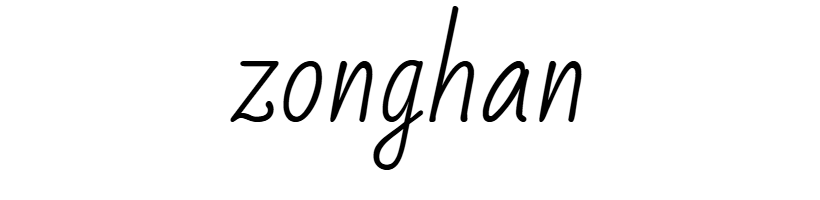
\includegraphics[height=1.2cm]{../Signatures/signature_zonghan.jpg}} \\
\hline
Lin Yuhao & BDST-RE-BA-003 & \makebox[\linewidth][c]{
\includegraphics[height=1.2cm]{../Signatures/signature_yuhao.jpg}} \\
\hline
Muhammad Mikhail Bin Mazlan & BDST-RE-BA-004 & \makebox[\linewidth][c]{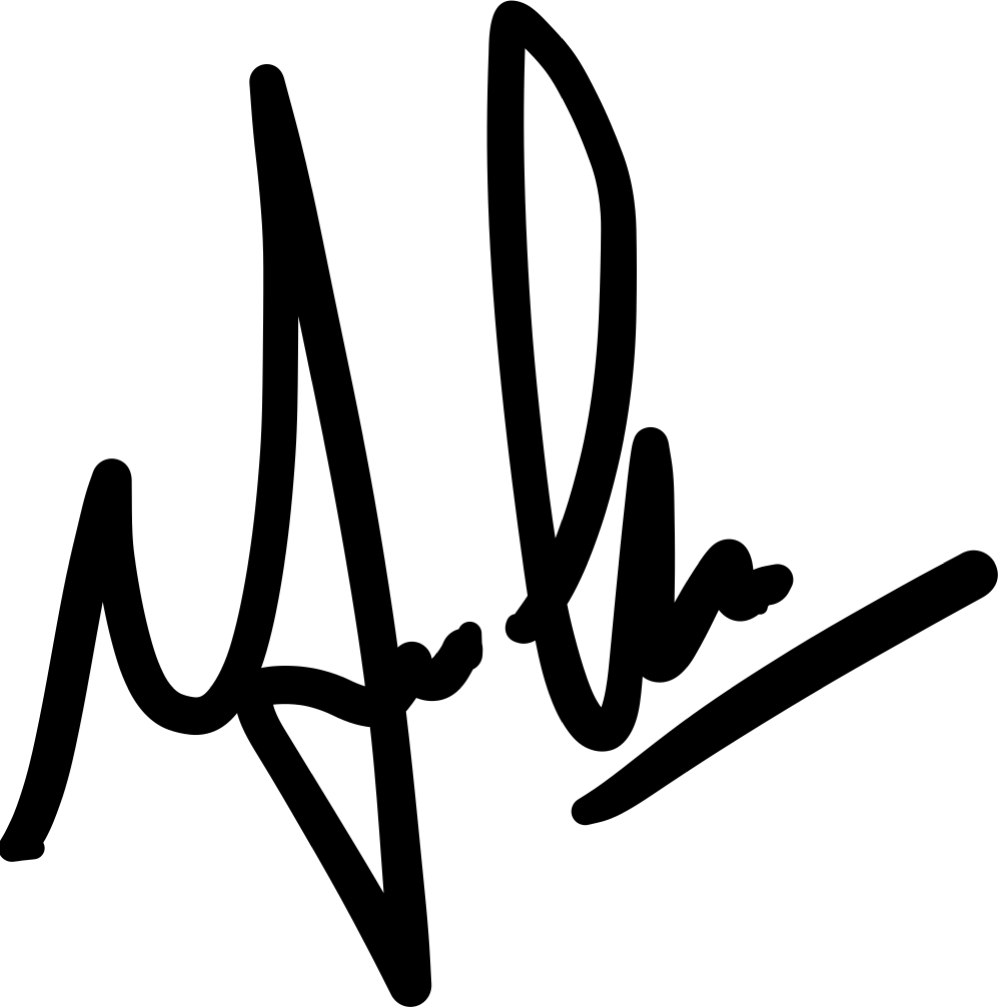
\includegraphics[height=1.2cm]{../Signatures/signature_mikhail.jpg}} \\
\hline
Kannan s/o Rajamohan & BDST-RE-BA-005 & \makebox[\linewidth][c]{
\includegraphics[height=1.2cm]{../Signatures/signature_kannan.jpg}} \\
\hline
\end{tabular}
\caption{Vendor team sign-off (signatures provided)}
\label{tab:vendor-signoff}
\end{table}

\subsection{Designated Approvers}
\begin{table}[H]
\centering
\small
\renewcommand{\arraystretch}{1.2}
\begin{tabular}{|p{0.17\textwidth}|p{0.29\textwidth}|p{0.24\textwidth}|p{0.2\textwidth}|}
\hline
\rowcolor{tableheader}
\textbf{Organization} & \textbf{Role} & \textbf{Name (Designated)} & \textbf{Signature (Designated)} \\
\hline
Customer (Triton Deepwater) & Project Leader / Requirements Approver & Sarah Whitman & \makebox[\linewidth][c]{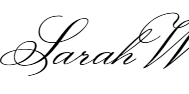
\includegraphics[height=1.2cm]{../Signatures/sarah_whitman.png}} \\
\hline
Customer (Triton Deepwater) & Safety \& Compliance Approver & Emily Carter & \makebox[\linewidth][c]{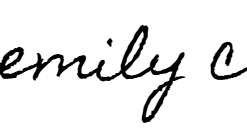
\includegraphics[height=1.2cm]{../Signatures/emily_carter.png}} \\
\hline
Vendor (Brigman Deep Sea Technology) & Engineering Delivery Lead & Nathan Briggs & \makebox[\linewidth][c]{
\includegraphics[height=1.2cm]{../Signatures/Briggman_Sig.png}} \\
\hline
Vendor (Brigman Deep Sea Technology) & Verification \& Validation Lead & Olivia Reyes & \makebox[\linewidth][c]{
\includegraphics[height=1.2cm]{../Signatures/Olivia_Sig.png}} \\
\hline
\end{tabular}
\caption{Designated approvers (named individuals; executed signatures recorded in formal approval transmittal)}
\label{tab:designated-approvers}
\end{table}

\smallskip
\noindent\textit{Named designated approvers and signature are maintained in this SRS baseline for governance visibility. Executed signatures may be recorded or updated in formal approval transmittal documentation. Approval authority remains role-based to preserve governance continuity across personnel changes.}

% =====================
% 12. DECLARATIONS
% =====================
\section{Declarations}
\label{sec:declarations}

\textbf{AI Tool Usage Declaration:} We acknowledge the use of AI tools (including ChatGPT) to assist with language refinement, structural organisation, and clarity of presentation. Prompts were used to review section structure, improve wording, and improve document flow. The output was used solely to refine phrasing and presentation. We confirm that no AI-generated analytical content, traceability decisions, models, or technical conclusions have been presented as our own work. All requirements analysis, codification, and validation were performed by the team.

\textbf{Originality Declaration:} This Software Requirements Specification presents original requirements work by Brigman Deep Sea Technology. The BCIC framework is a proprietary methodology invented by Dr Kevin Anthony Jones and applied by us specifically to this project. All sources are cited in the References section.

\textbf{Software Compliance Declaration:} This SRS aligns with IEEE 830 principles and applies CRaM criteria (Correct, Relevant, Measurable) throughout requirements specification.

\textbf{Software Scope Declaration:} This SRS covers software requirements only. Hardware specifications and physical interfaces are customer-defined; the software integrates those components within the defined system boundary.

\textbf{Academic Integrity Declaration:} No plagiarism, unauthorised collaboration, or academic misconduct occurred in the preparation of this document.

\section*{Repository Information}
\addcontentsline{toc}{section}{Repository Information}
\begin{center}
\fbox{\begin{minipage}{0.9\textwidth}
\centering
\textbf{PROJECT REPOSITORY}\\[2pt]
\href{https://github.com/Spooky312/The-Abyss-Navigation-Suite-INF2113}{\uline{\nolinkurl{https://github.com/Spooky312/The-Abyss-Navigation-Suite-INF2113}}}\\[4pt]
\textit{SRS, models, and traceability artifacts maintained under version control}
\end{minipage}}
\end{center}

% =====================
% References
% =====================
\clearpage
\pagenumbering{arabic}
\setcounter{page}{1}
\renewcommand{\thepage}{R-\arabic{page}}
\section*{References}
\addcontentsline{toc}{section}{References}
\begin{itemize}[leftmargin=*,nosep]
  \item Triton Deepwater, \textit{Project Specification: The Abyss Navigator Suite}, ICT2113, 2026.
  \item Brigman Deep Sea Technology, \textit{Software Requirements Analysis Report (BCIC Methodology)}, 2026.
  \item Kevin Anthony Jones, \textit{Labtorial Guide for Class Project: Reqrs now \& near future}, Dec 2025.
  \item Kevin Anthony Jones, \textit{Guide Rubric for Assessment of Deliverables}, Jan 2026.
  \item Karl E. Wiegers, \textit{Software Requirements Specification Template}, 1999.
\end{itemize}

% =====================
% Glossary
% =====================
\clearpage
\pagenumbering{arabic}
\setcounter{page}{1}
\renewcommand{\thepage}{G-\arabic{page}}
\section*{Glossary}
\addcontentsline{toc}{section}{Glossary}
\begin{description}[leftmargin=*,style=nextline,font=\normalfont\bfseries]
  \item[AES-256] Advanced Encryption Standard with 256-bit key length used for data encryption at rest and in transit.
  \item[Anomaly Alert] A system-generated notification triggered when operational parameters deviate beyond defined thresholds.
  \item[Append-Only Log] A logging mechanism where records can only be added and not modified or deleted, ensuring audit integrity.
  \item[Autonomous Execution] Mission execution performed without continuous human control, based on pre-configured mission plans.
  \item[Baseline (SRS Baseline)] The formally approved version of this SRS used as the reference point for design, implementation, and change control.
  \item[BCIC] Breakdown, Clarify, Interpret, Categorize — the requirements derivation method applied in this SRS.
  \item[Blackbox Logging] Redundant logging mechanism storing critical operational data both onboard the submersible and on the mothership for post-incident analysis.
  \item[CHG-\textlangle AREA\textrangle-\textlangle NNN\textrangle] Codification scheme used for change mitigation controls in Section 8.
  \item[COM-DEG-001] Requirement governing degraded communication handling and safe-state triggering under communication loss.
  \item[Constrained Communications] Operational context characterised by low bandwidth, high latency, and intermittent connectivity.
  \item[Contingency Control (CHG-CONT-*)] Pre-approved change control triggered by anticipated conditions such as regulatory updates or integration mismatches.
  \item[CRaM] Correct, Relevant, and Measurable — requirements organisation principle applied throughout this SRS.
  \item[DDS (Data Distribution Service)] Middleware transport protocol used for real-time, reliable, and scalable data exchange in distributed systems.
  \item[Degraded Mode] Operational state in which the mission continues with limited functionality while alerting operators and logging the condition.
  \item[Emergency Retrieval] Autonomous system-initiated ascent and recovery process triggered under catastrophic conditions.
  \item[Fault Injection] Testing technique involving deliberate introduction of faults to verify detection and recovery behaviour.
  \item[iRTM (Integrated Requirements Traceability Matrix)] Artifact mapping Project Specification clauses to SRS requirements, ensuring bidirectional traceability.
  \item[JSON Schema] Structured data definition format used for defining and validating message payloads.
  \item[McCall Quality Model] Software quality framework organising quality into Product Operation, Product Revision, and Product Transition perspectives.
  \item[Mission Plan] Version-controlled structured definition of waypoints and mission phases for autonomous execution.
  \item[Mission Run] An instantiated execution of a mission plan with runtime state tracking.
  \item[Mutual Authentication] Security mechanism requiring both communicating parties to validate each other using digital certificates.
  \item[Normative Language (``Shall'')] Mandatory wording used to indicate enforceable requirements.
  \item[Open Issue Control (CHG-OISS-*)] Codified unresolved requirement item tracked with a responsible party and kill date.
  \item[Operational Log Record] Timestamped record of mission or operator activity including attribution and severity classification.
  \item[Product Specification (PS)] Customer-issued specification forming the source baseline for vendor requirement derivation.
  \item[QUAL-\textlangle AREA\textrangle-\textlangle NNN\textrangle] Codification scheme for BDST Quality Model features aligned with McCall's model.
  \item[Requirement ID Stability Rule] Rule stating that requirement identifiers remain unchanged across revisions to preserve traceability.
  \item[Role-Based Access Control (RBAC)] Access control mechanism restricting permissions based on assigned user roles.
  \item[ROS2] Robot Operating System version 2 middleware framework supporting distributed robotics applications.
  \item[Safe-State] Defined operational condition characterised by neutral buoyancy, minimal power consumption, and active communication beacon.
  \item[SDLC (Software Development Life Cycle)] Structured lifecycle including requirements, design, implementation, verification, and maintenance phases.
  \item[SEC-AUD-001] Requirement governing audit logging for access and configuration changes.
  \item[SEC-AUTH-001] Requirement governing X.509-based mutual authentication.
  \item[SEC-ENC-001] Requirement governing encryption of operational data.
  \item[Session Timeout] Security mechanism automatically terminating inactive sessions after a configured duration.
  \item[Specifying Method (Vendor Provision)] Requirements introduced by the vendor beyond the PS baseline (technology stack, quality model, governance).
  \item[Trace Type (DT\,/\,AT\,/\,VP)] Classification used in the iRTM: \textbf{DT} -- Direct Trace; \textbf{AT} -- Assumption Trace; \textbf{VP} -- Vendor Provision.
  \item[Two-Factor Authentication (2FA)] Authentication mechanism requiring two independent verification factors.
  \item[UDS (Unmanned Deep-sea Submersible)] The autonomous deep-sea platform controlled by the Abyss Navigator Suite.
  \item[UTC (Coordinated Universal Time)] Standardised time reference used for all timestamped logs and mission records.
  \item[Vendor Provision (VP)] Requirement introduced by the vendor under the Specifying method rather than directly derived from the PS.
\end{description}
% =====================
% TBD List
% =====================
\clearpage
\pagenumbering{arabic}
\setcounter{page}{1}
\renewcommand{\thepage}{T-\arabic{page}}
\section*{To Be Determined (TBD) List}
\addcontentsline{toc}{section}{To Be Determined (TBD) List}
\begin{itemize}[leftmargin=*,nosep]
  \item Final selection of database product/version for TECH-DB-001 (if different from PostgreSQL-equivalent).
  \item Final JSON schemas for INT-SENS-001 (to be published with the Interface/API guide).
\end{itemize}

% =====================
% FIGURES 
% =====================
\clearpage
\pagenumbering{arabic}
\setcounter{page}{1}
\renewcommand{\thepage}{F-\arabic{page}}
\section*{Figures}
\addcontentsline{toc}{section}{Figures}
\label{sec:figures}

\addtocounter{figure}{0}

\begin{figure}[H]
\centering
\orighyperref[tab:response-sequence]{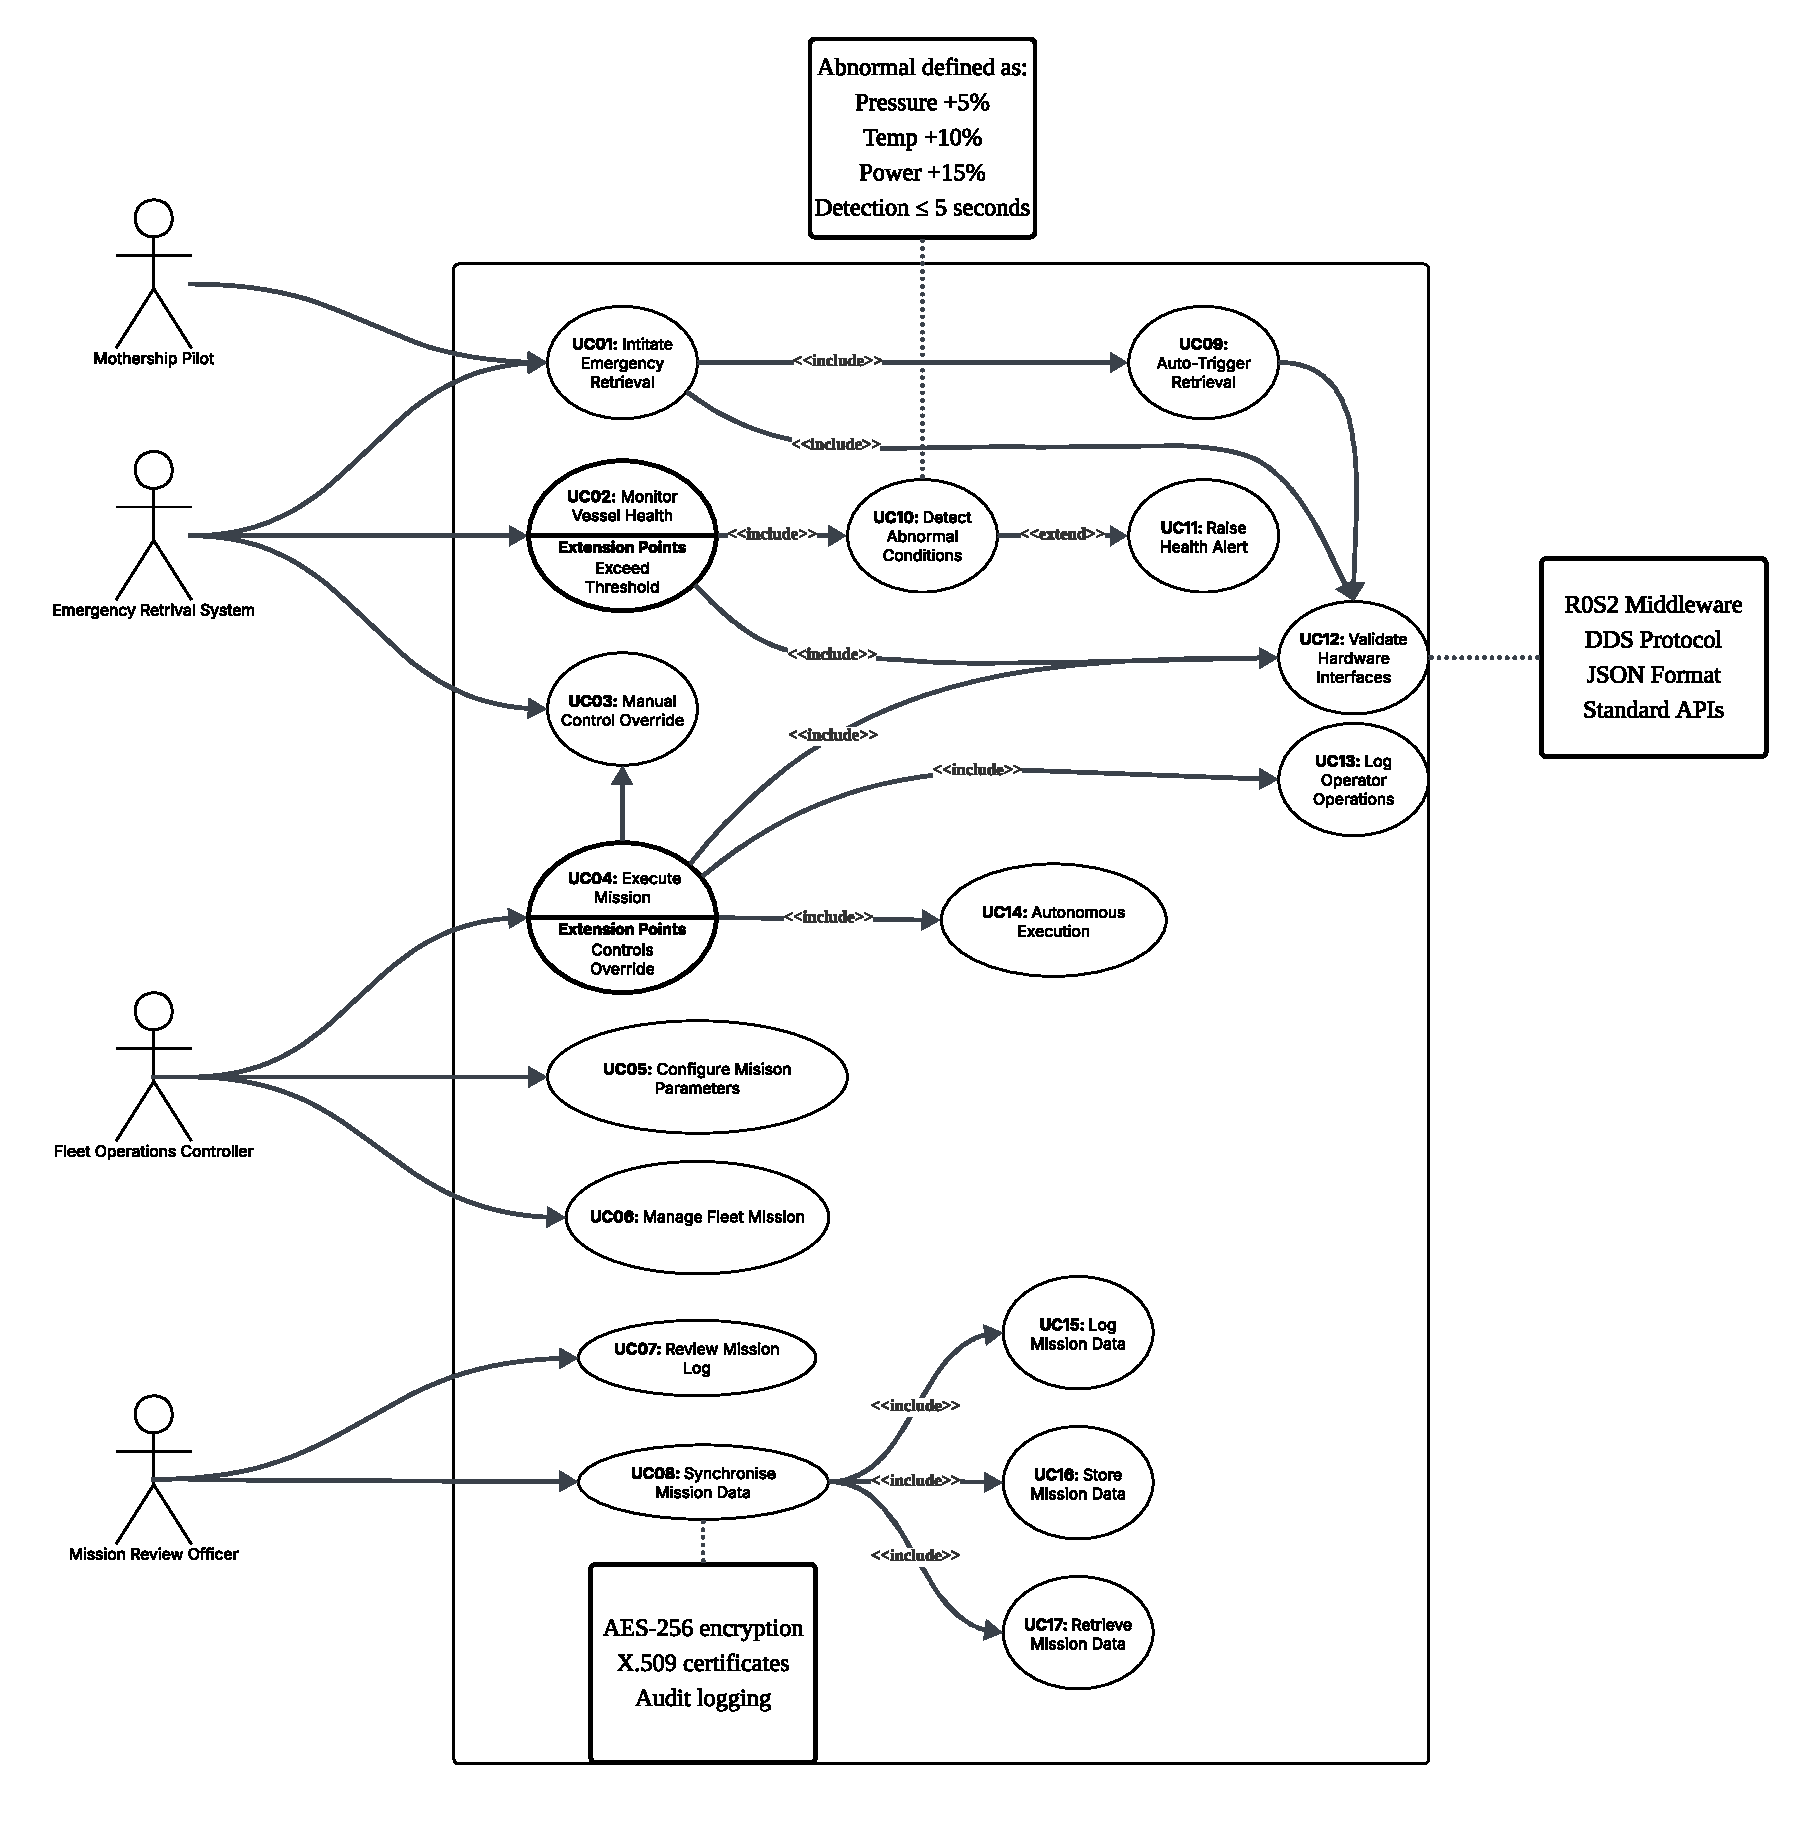
\includegraphics[width=0.95\textwidth]{../Models/Use Case Diagram.pdf}}
\caption{Use Case Diagram}
\label{fig:usecase-diagram-pdf}
\end{figure}

\subsection*{Instructions}
The diagram illustrates the primary actors (surface controller, mothership crew, autonomous submersible) and 
their interactions with major system functions such as mission planning, launch/recovery, sensor telemetry, 
fault handling, and data logging. Follow each actor’s swim lane to see how the mission progresses 
from preparation to post-mission data review; the colored connectors highlight safety-critical flows 
(emergency surfacing, manual override) that must remain available throughout operations.

\vspace{1em}




% ---- Appendix page prefix helper (A-1, B-1, C-1...) ----
\newcommand{\startappendix}[2]{%
  \setcounter{page}{1}%
  \renewcommand{\thepage}{#1-\arabic{page}}%
  \setcounter{table}{0}%
  \renewcommand{\thetable}{#1-\arabic{table}}%
  \section*{Appendix #1: #2}%
  \addcontentsline{toc}{section}{Appendix #1: #2}%
  \phantomsection
}

% =====================
% APPENDICES (Main Header)
% =====================
\clearpage
\section*{APPENDICES}
\addcontentsline{toc}{section}{APPENDICES}
\phantomsection
% --------------------
% Appendix A: Data Dictionary
% --------------------
\startappendix{A}{Data Dictionary}
\label{app:data-dictionary}

This section defines the data entities used by the system and the attributes that describe each entity.

% ====================
% Entity: Operator
% ====================
\begin{table}[H]
\centering
\small
\renewcommand{\arraystretch}{1.2}
\begin{tabular}{|>{\raggedright\arraybackslash}p{0.18\textwidth}|>{\raggedright\arraybackslash}p{0.14\textwidth}|>{\raggedright\arraybackslash}p{0.10\textwidth}|>{\raggedright\arraybackslash}p{0.26\textwidth}|>{\raggedright\arraybackslash}p{0.22\textwidth}|}
\hline
\multicolumn{5}{|l|}{\textbf{\hyperref[flow-Operator]{Entity: Operator}}} \\
\hline
\rowcolor{tableheader}
\textbf{Attribute} & \textbf{Data Type} & \textbf{Length} & \textbf{Constraints} & \textbf{Description} \\
\hline
OperatorID & VARCHAR & 20 & PK, NOT NULL, UNIQUE & Unique operator identifier used in UI (e.g., OP-2847) \\
\hline
Username & VARCHAR & 50 & NOT NULL, UNIQUE & Login username / operator ID entry \\
\hline
FullName & VARCHAR & 100 & NOT NULL & Display name shown in admin list \\
\hline
Role & ENUM & - &
\begin{tabular}[t]{@{}l@{}}
'Fleet Operator',\\
'Mission Supervisor',\\
'Safety \& Compliance Officer',\\
'Data Analyst',\\
'System Administrator'
\end{tabular} & Selected user role \\
\hline
AccountStatus & ENUM & - &
\begin{tabular}[t]{@{}l@{}}
'Active',\\
'Inactive',\\
'Locked',\\
'Disabled'
\end{tabular} & Account status shown in admin UI \\
\hline
TwoFactorEnabled & BOOLEAN & - & NOT NULL, DEFAULT FALSE & Whether 2FA is enabled for this user \\
\hline
LastLoginUTC & TIMESTAMP & - & NULL & Last successful login time (UTC) \\
\hline
CreatedAtUTC & TIMESTAMP & - & NOT NULL & Record creation time (UTC) \\
\hline
\end{tabular}
\caption{Data dictionary for \textbf{Operator} entity}
\label{tab:data-dictionary-operator}
\end{table}

% ====================
% Entity: LoginSession
% ====================
\begin{table}[H]
\centering
\small
\renewcommand{\arraystretch}{1.2}
\begin{tabular}{|>{\raggedright\arraybackslash}p{0.18\textwidth}|>{\raggedright\arraybackslash}p{0.14\textwidth}|>{\raggedright\arraybackslash}p{0.10\textwidth}|>{\raggedright\arraybackslash}p{0.26\textwidth}|>{\raggedright\arraybackslash}p{0.22\textwidth}|}
\hline
\multicolumn{5}{|l|}{\textbf{\hyperref[flow-LoginSession]{Entity: LoginSession}}} \\
\hline
\rowcolor{tableheader}
\textbf{Attribute} & \textbf{Data Type} & \textbf{Length} & \textbf{Constraints} & \textbf{Description} \\
\hline
SessionID & VARCHAR & 36 & PK, NOT NULL, UNIQUE & Unique session identifier \\
\hline
OperatorID & VARCHAR & 20 & \begin{tabular}[t]{@{}l@{}}FK $\rightarrow$ Operator.OperatorID,\\ NOT NULL\end{tabular} & Logged-in user \\
\hline
LoginUTC & TIMESTAMP & - & NOT NULL & Login timestamp (UTC) \\
\hline
LogoutUTC & TIMESTAMP & - & NULL & Logout timestamp (UTC) \\
\hline
TwoFactorVerified & BOOLEAN & - & NOT NULL & Whether 2FA verification succeeded \\
\hline
SessionStatus & ENUM & - &
\begin{tabular}[t]{@{}l@{}}
'Active',\\
'Expired',\\
'Terminated'
\end{tabular} & Session state \\
\hline
IPAddress & VARCHAR & 45 & NULL & Optional login source IP address \\
\hline
\end{tabular}
\caption{Data dictionary for \textbf{LoginSession} entity}
\label{tab:data-dictionary-loginsession}
\end{table}

% ====================
% Entity: Vehicle
% ====================
\begin{table}[H]
\centering
\small
\renewcommand{\arraystretch}{1.2}
\begin{tabular}{|>{\raggedright\arraybackslash}p{0.18\textwidth}|>{\raggedright\arraybackslash}p{0.14\textwidth}|>{\raggedright\arraybackslash}p{0.10\textwidth}|>{\raggedright\arraybackslash}p{0.26\textwidth}|>{\raggedright\arraybackslash}p{0.22\textwidth}|}
\hline
\multicolumn{5}{|l|}{\centering\textbf{\hyperref[flow-Vehicle]{Entity: Vehicle}}} \\
\hline
\rowcolor{tableheader}
\textbf{Attribute} & \textbf{Data Type} & \textbf{Length} & \textbf{Constraints} & \textbf{Description} \\
\hline
VehicleID & VARCHAR & 20 & PK, NOT NULL, UNIQUE & Vehicle identifier shown in UI (e.g., ASV-01) \\
\hline
DisplayName & VARCHAR & 100 & NOT NULL & Vehicle name shown (e.g., Deep Explorer) \\
\hline
OperationalStatus & ENUM & - &
\begin{tabular}[t]{@{}l@{}}
'Active',\\
'Paused',\\
'Safe-State'
\end{tabular} & Status shown on vehicle card \\
\hline
CurrentDepth\_m & DECIMAL & (8,2) & NULL & Current depth (meters) shown on vehicle card \\
\hline
CurrentPower\_pct & DECIMAL & (5,2) & NULL & Current power (percent) shown on vehicle card \\
\hline
CurrentPressure\_bar & DECIMAL & (7,2) & NULL & Current pressure (bar) shown on vehicle card \\
\hline
CurrentTemp\_c & DECIMAL & (5,2) & NULL & Current temperature (Celsius) shown on vehicle card \\
\hline
LastKnownLat & DECIMAL & (10,6) & NULL & Last known latitude \\
\hline
LastKnownLon & DECIMAL & (10,6) & NULL & Last known longitude \\
\hline
LastUpdateUTC & TIMESTAMP & - & NULL & Last telemetry update time (UTC) \\
\hline
\end{tabular}
\caption{Data dictionary for \textbf{Vehicle} entity}
\label{tab:data-dictionary-vehicle}
\end{table}

% ====================
% Entity: MissionPlan
% ====================
\begin{table}[H]
\centering
\small
\renewcommand{\arraystretch}{1.2}
\begin{tabular}{|>{\raggedright\arraybackslash}p{0.18\textwidth}|>{\raggedright\arraybackslash}p{0.14\textwidth}|>{\raggedright\arraybackslash}p{0.10\textwidth}|>{\raggedright\arraybackslash}p{0.26\textwidth}|>{\raggedright\arraybackslash}p{0.22\textwidth}|}
\hline
\multicolumn{5}{|l|}{\centering\textbf{\hyperref[flow-MissionPlan]{Entity: MissionPlan}}} \\
\hline
\rowcolor{tableheader}
\textbf{Attribute} & \textbf{Data Type} & \textbf{Length} & \textbf{Constraints} & \textbf{Description} \\
\hline
MissionPlanID & VARCHAR & 36 & PK, NOT NULL, UNIQUE & Unique mission plan identifier \\
\hline
MissionName & VARCHAR & 120 & NOT NULL & Mission name shown in UI (e.g., Hydrothermal Survey 12B) \\
\hline
Version & VARCHAR & 10 & NOT NULL & Mission plan version (e.g., 1.3) \\
\hline
TargetVehicleID & VARCHAR & 20 & \begin{tabular}[t]{@{}l@{}}FK $\rightarrow$ Vehicle.VehicleID,\\ NOT NULL\end{tabular} & Selected target vehicle \\
\hline
Estimated\allowbreak DurationHours & DECIMAL & (4,1) & NULL & Estimated duration (hours) shown in UI \\
\hline
Status & ENUM & - &
\begin{tabular}[t]{@{}l@{}}
'Draft',\\
'Deployed',\\
'Archived'
\end{tabular} & Mission plan status shown in summary \\
\hline
CreatedBy & VARCHAR & 20 & \begin{tabular}[t]{@{}l@{}}FK $\rightarrow$ Operator.OperatorID,\\ NOT NULL\end{tabular} & Creator of the plan \\
\hline
CreatedAtUTC & TIMESTAMP & - & NOT NULL & Creation time (UTC) \\
\hline
UpdatedAtUTC & TIMESTAMP & - & NULL & Last update time (UTC) \\
\hline
\end{tabular}
\caption{Data dictionary for \textbf{MissionPlan} entity}
\label{tab:data-dictionary-missionplan}
\end{table}

% ====================
% Entity: Waypoint 
% ====================
\begin{table}[H]
\centering
\small
\renewcommand{\arraystretch}{1.2}
\begin{tabular}{|>{\raggedright\arraybackslash}p{0.18\textwidth}|>{\raggedright\arraybackslash}p{0.14\textwidth}|>{\raggedright\arraybackslash}p{0.10\textwidth}|>{\raggedright\arraybackslash}p{0.26\textwidth}|>{\raggedright\arraybackslash}p{0.22\textwidth}|}
\hline
\multicolumn{5}{|l|}{\centering\textbf{\hyperref[flow-Waypoint]{Entity: Waypoint }}} \\
\hline
\rowcolor{tableheader}
\textbf{Attribute} & \textbf{Data Type} & \textbf{Length} & \textbf{Constraints} & \textbf{Description} \\
\hline
WaypointID & VARCHAR & 36 & PK, NOT NULL, UNIQUE & Unique waypoint identifier \\
\hline
MissionPlanID & VARCHAR & 36 & \begin{tabular}[t]{@{}l@{}}FK $\rightarrow$ MissionPlan.\\ MissionPlanID,\\ NOT NULL\end{tabular} & Mission plan this waypoint belongs to \\
\hline
SequenceNo & INTEGER & 5 & NOT NULL & Waypoint order (supports reordering in UI) \\
\hline
Latitude & DECIMAL & (10,6) & NOT NULL & Waypoint latitude \\
\hline
Longitude & DECIMAL & (10,6) & NOT NULL & Waypoint longitude \\
\hline
Depth\_m & DECIMAL & (8,2) & NOT NULL & Target depth at this waypoint (meters) \\
\hline
Phase & ENUM & - &
\begin{tabular}[t]{@{}l@{}}
'Transit',\\
'Survey',\\
'Sample'
\end{tabular} & Operational phase selected in UI \\
\hline
\end{tabular}
\caption{Data dictionary for \textbf{Waypoint} entity}
\label{tab:data-dictionary-waypoint}
\end{table}

% ====================
% Entity: MissionRun 
% ====================
\begin{table}[H]
\centering
\small
\renewcommand{\arraystretch}{1.2}
\begin{tabular}{|>{\raggedright\arraybackslash}p{0.18\textwidth}|>{\raggedright\arraybackslash}p{0.14\textwidth}|>{\raggedright\arraybackslash}p{0.10\textwidth}|>{\raggedright\arraybackslash}p{0.26\textwidth}|>{\raggedright\arraybackslash}p{0.22\textwidth}|}
\hline
\multicolumn{5}{|l|}{\centering\textbf{\hyperref[flow-MissionRun]{Entity: MissionRun}}} \\
\hline
\rowcolor{tableheader}
\textbf{Attribute} & \textbf{Data Type} & \textbf{Length} & \textbf{Constraints} & \textbf{Description} \\
\hline
MissionID & VARCHAR & 36 & PK, NOT NULL, UNIQUE & Unique mission execution identifier \\
\hline
MissionPlanID & VARCHAR & 36 & \begin{tabular}[t]{@{}l@{}}FK $\rightarrow$ MissionPlan.\\ MissionPlanID,\\ NOT NULL\end{tabular} & Mission plan deployed \\
\hline
VehicleID & VARCHAR & 20 & \begin{tabular}[t]{@{}l@{}}FK $\rightarrow$ Vehicle.VehicleID,\\ NOT NULL\end{tabular} & Vehicle executing mission \\
\hline
StartUTC & TIMESTAMP & - & NOT NULL & Mission start time (UTC) \\
\hline
EndUTC & TIMESTAMP & - & NULL & Mission end time (UTC) \\
\hline
State & ENUM & - &
\begin{tabular}[t]{@{}l@{}}
'Running',\\
'Completed',\\
'Paused',\\
'Safe-State',\\
'Terminated'
\end{tabular} & Mission execution state \\
\hline
WaypointSuccess\_\allowbreak pct & DECIMAL & (5,2) & NULL & Waypoint success rate (percent) \\
\hline
\end{tabular}
\caption{Data dictionary for \textbf{MissionRun} entity}
\label{tab:data-dictionary-missionrun}
\end{table}

% ====================
% Entity: TelemetrySnapshot
% ====================
\begin{table}[H]
\centering
\small
\renewcommand{\arraystretch}{1.2}
\begin{tabular}{|>{\raggedright\arraybackslash}p{0.18\textwidth}|>{\raggedright\arraybackslash}p{0.14\textwidth}|>{\raggedright\arraybackslash}p{0.10\textwidth}|>{\raggedright\arraybackslash}p{0.26\textwidth}|>{\raggedright\arraybackslash}p{0.22\textwidth}|}
\hline
\multicolumn{5}{|l|}{\centering\textbf{\hyperref[flow-TelemetrySnapshot]{Entity: TelemetrySnapshot}}} \\
\hline
\rowcolor{tableheader}
\textbf{Attribute} & \textbf{Data Type} & \textbf{Length} & \textbf{Constraints} & \textbf{Description} \\
\hline
TelemetryID & VARCHAR & 36 & PK, NOT NULL, UNIQUE & Unique telemetry record \\
\hline
MissionID & VARCHAR & 36 & \begin{tabular}[t]{@{}l@{}}FK $\rightarrow$ MissionRun.MissionID,\\ NOT NULL\end{tabular} & Mission reference \\
\hline
VehicleID & VARCHAR & 20 & \begin{tabular}[t]{@{}l@{}}FK $\rightarrow$ Vehicle.VehicleID,\\ NOT NULL\end{tabular} & Vehicle reference \\
\hline
TimestampUTC & TIMESTAMP & - & NOT NULL & Time telemetry recorded (UTC) \\
\hline
Depth\_m & DECIMAL & (8,2) & NOT NULL & Depth (meters) shown on vehicle card \\
\hline
Power\_pct & DECIMAL & (5,2) & NOT NULL & Power (percent) shown on vehicle card \\
\hline
Pressure\_bar & DECIMAL & (7,2) & NOT NULL & Pressure (bar) shown on vehicle card \\
\hline
Temp\_c & DECIMAL & (5,2) & NOT NULL & Temperature (Celsius) shown on vehicle card \\
\hline
Latitude & DECIMAL & (10,6) & NOT NULL & Latitude shown on vehicle card and map \\
\hline
Longitude & DECIMAL & (10,6) & NOT NULL & Longitude shown on vehicle card and map \\
\hline
PayloadJSON & JSON & - & NULL & Optional raw payload for extensibility \\
\hline
\end{tabular}
\caption{Data dictionary for \textbf{TelemetrySnapshot} entity}
\label{tab:data-dictionary-telemetrysnapshot}
\end{table}

% ====================
% Entity: CommsLinkSnapshot
% ====================
\begin{table}[H]
\centering
\small
\renewcommand{\arraystretch}{1.2}
\begin{tabular}{|>{\raggedright\arraybackslash}p{0.18\textwidth}|>{\raggedright\arraybackslash}p{0.14\textwidth}|>{\raggedright\arraybackslash}p{0.10\textwidth}|>{\raggedright\arraybackslash}p{0.26\textwidth}|>{\raggedright\arraybackslash}p{0.22\textwidth}|}
\hline
\multicolumn{5}{|l|}{\centering\textbf{\hyperref[flow-CommsLinkSnapshot]{Entity: CommsLinkSnapshot}}} \\
\hline
\rowcolor{tableheader}
\textbf{Attribute} & \textbf{Data Type} & \textbf{Length} & \textbf{Constraints} & \textbf{Description} \\
\hline
LinkSnapID & VARCHAR & 36 & PK, NOT NULL, UNIQUE & Unique communications snapshot \\
\hline
MissionID & VARCHAR & 36 & \begin{tabular}[t]{@{}l@{}}FK $\rightarrow$ MissionRun.MissionID,\\ NOT NULL\end{tabular} & Mission reference \\
\hline
TimestampUTC & TIMESTAMP & - & NOT NULL & Snapshot time (UTC) \\
\hline
LinkType & ENUM & - &
\begin{tabular}[t]{@{}l@{}}
'Satellite',\\
'Acoustic',\\
'RF'
\end{tabular} & Communication link type used \\
\hline
ConnectionStatus & ENUM & - &
\begin{tabular}[t]{@{}l@{}}
'Connected',\\
'Degraded',\\
'Disconnected'
\end{tabular} & Link connection status \\
\hline
LinkQuality\_pct & DECIMAL & (5,2) & NOT NULL & Link quality (percent) shown in UI \\
\hline
Bandwidth\_mbps & DECIMAL & (6,2) & NOT NULL & Bandwidth (Mbps) shown in UI \\
\hline
Latency\_ms & INTEGER & 6 & NOT NULL & Latency (ms) shown in UI \\
\hline
\end{tabular}
\caption{Data dictionary for \textbf{CommsLinkSnapshot} entity}
\label{tab:data-dictionary-commslinksnapshot}
\end{table}

% ====================
% Entity: InterventionCommand
% ====================
\begin{table}[H]
\centering
\small
\renewcommand{\arraystretch}{1.2}
\begin{tabular}{|>{\raggedright\arraybackslash}p{0.18\textwidth}|>{\raggedright\arraybackslash}p{0.14\textwidth}|>{\raggedright\arraybackslash}p{0.10\textwidth}|>{\raggedright\arraybackslash}p{0.26\textwidth}|>{\raggedright\arraybackslash}p{0.22\textwidth}|}
\hline
\multicolumn{5}{|l|}{\centering\textbf{\hyperref[flow-InterventionCommand]{Entity: InterventionCommand}}} \\
\hline
\rowcolor{tableheader}
\textbf{Attribute} & \textbf{Data Type} & \textbf{Length} & \textbf{Constraints} & \textbf{Description} \\
\hline
CommandID & VARCHAR & 36 & PK, NOT NULL, UNIQUE & Unique command identifier \\
\hline
MissionID & VARCHAR & 36 & \begin{tabular}[t]{@{}l@{}}FK $\rightarrow$ MissionRun.MissionID,\\ NOT NULL\end{tabular} & Related mission \\
\hline
TargetVehicleID & VARCHAR & 20 & \begin{tabular}[t]{@{}l@{}}FK $\rightarrow$ Vehicle.VehicleID,\\ NOT NULL\end{tabular} & Vehicle receiving the command \\
\hline
IssuedBy & VARCHAR & 20 & \begin{tabular}[t]{@{}l@{}}FK $\rightarrow$ Operator.OperatorID,\\ NOT NULL\end{tabular} & Operator who issued the command \\
\hline
CommandType & ENUM & - &
\begin{tabular}[t]{@{}l@{}}
'Pause',\\
'Resume',\\
'Safe-State'
\end{tabular} & Command type from the dashboard controls \\
\hline
IssuedAtUTC & TIMESTAMP & - & NOT NULL & Command issued time (UTC) \\
\hline
CommandStatus & ENUM & - &
\begin{tabular}[t]{@{}l@{}}
'Sent',\\
'Acknowledged',\\
'Failed'
\end{tabular} & Command delivery outcome \\
\hline
AckReceivedAtUTC & TIMESTAMP & - & NULL & Acknowledgement received time (UTC) \\
\hline
FailureReason & VARCHAR & 255 & NULL & Reason if command failed \\
\hline
\end{tabular}
\caption{Data dictionary for \textbf{InterventionCommand} entity}
\label{tab:data-dictionary-interventioncommand}
\end{table}

% ====================
% Entity: BaselineProfile
% ====================
\begin{table}[H]
\centering
\small
\renewcommand{\arraystretch}{1.2}
\begin{tabular}{|>{\raggedright\arraybackslash}p{0.18\textwidth}|>{\raggedright\arraybackslash}p{0.14\textwidth}|>{\raggedright\arraybackslash}p{0.10\textwidth}|>{\raggedright\arraybackslash}p{0.26\textwidth}|>{\raggedright\arraybackslash}p{0.22\textwidth}|}
\hline
\multicolumn{5}{|l|}{\centering\textbf{\hyperref[flow-BaselineProfile]{Entity: BaselineProfile}}} \\
\hline
\rowcolor{tableheader}
\textbf{Attribute} & \textbf{Data Type} & \textbf{Length} & \textbf{Constraints} & \textbf{Description} \\
\hline
BaselineID & VARCHAR & 36 & PK, NOT NULL, UNIQUE & Baseline profile identifier \\
\hline
VehicleID & VARCHAR & 20 & \begin{tabular}[t]{@{}l@{}}FK $\rightarrow$ Vehicle.VehicleID,\\ NOT NULL\end{tabular} & Vehicle baseline applies to \\
\hline
MetricType & ENUM & - &
\begin{tabular}[t]{@{}l@{}}
'Power',\\
'Pressure',\\
'Temp'
\end{tabular} & Metric being compared against baseline \\
\hline
BaselineValue & DECIMAL & (8,2) & NOT NULL & Baseline reference value \\
\hline
EffectiveFromUTC & TIMESTAMP & - & NOT NULL & Start of validity (UTC) \\
\hline
EffectiveToUTC & TIMESTAMP & - & NULL & End of validity (UTC) \\
\hline
\end{tabular}
\caption{Data dictionary for \textbf{BaselineProfile} entity}
\label{tab:data-dictionary-baselineprofile}
\end{table}

% ====================
% Entity: AnomalyAlert
% ====================
\begin{table}[H]
\centering
\small
\renewcommand{\arraystretch}{1.2}
\begin{tabular}{|>{\raggedright\arraybackslash}p{0.18\textwidth}|>{\raggedright\arraybackslash}p{0.14\textwidth}|>{\raggedright\arraybackslash}p{0.10\textwidth}|>{\raggedright\arraybackslash}p{0.26\textwidth}|>{\raggedright\arraybackslash}p{0.22\textwidth}|}
\hline
\multicolumn{5}{|l|}{\centering\textbf{\hyperref[flow-AnomalyAlert]{Entity: AnomalyAlert}}} \\
\hline
\rowcolor{tableheader}
\textbf{Attribute} & \textbf{Data Type} & \textbf{Length} & \textbf{Constraints} & \textbf{Description} \\
\hline
AlertID & VARCHAR & 36 & PK, NOT NULL, UNIQUE & Unique anomaly alert identifier \\
\hline
MissionID & VARCHAR & 36 & \begin{tabular}[t]{@{}l@{}}FK $\rightarrow$ MissionRun.MissionID,\\ NOT NULL\end{tabular} & Mission where anomaly occurred \\
\hline
VehicleID & VARCHAR & 20 & \begin{tabular}[t]{@{}l@{}}FK $\rightarrow$ Vehicle.VehicleID,\\ NOT NULL\end{tabular} & Vehicle involved \\
\hline
AlertType & ENUM & - &
\begin{tabular}[t]{@{}l@{}}
'Power',\\
'Pressure',\\
'Temp',\\
'Comms'
\end{tabular} & Alert type \\
\hline
Deviation\_pct & DECIMAL & (6,2) & NOT NULL & Deviation from baseline (percent) \\
\hline
Severity & ENUM & - &
\begin{tabular}[t]{@{}l@{}}
'INFO',\\
'WARNING',\\
'CRITICAL'
\end{tabular} & Severity level shown in UI \\
\hline
DetectedAtUTC & TIMESTAMP & - & NOT NULL & Detection time (UTC) \\
\hline
Status & ENUM & - &
\begin{tabular}[t]{@{}l@{}}
'Open',\\
'Acknowledged',\\
'Resolved'
\end{tabular} & Alert lifecycle state \\
\hline
ReviewedBy & VARCHAR & 20 & \begin{tabular}[t]{@{}l@{}}FK $\rightarrow$ Operator.OperatorID,\\ NULL\end{tabular} & Operator who reviewed/responded \\
\hline
ReviewedAtUTC & TIMESTAMP & - & NULL & Review time (UTC) \\
\hline
\end{tabular}
\caption{Data dictionary for \textbf{AnomalyAlert} entity}
\label{tab:data-dictionary-anomalyalert}
\end{table}

% ====================
% Entity: OperationalLogRecord 
% ====================
\begin{table}[H]
\centering
\small
\renewcommand{\arraystretch}{1.2}
\begin{tabular}{|>{\raggedright\arraybackslash}p{0.18\textwidth}|>{\raggedright\arraybackslash}p{0.14\textwidth}|>{\raggedright\arraybackslash}p{0.10\textwidth}|>{\raggedright\arraybackslash}p{0.26\textwidth}|>{\raggedright\arraybackslash}p{0.22\textwidth}|}
\hline
\multicolumn{5}{|l|}{\centering\textbf{\hyperref[flow-OperationalLogRecord]{Entity: OperationalLogRecord}}} \\
\hline
\rowcolor{tableheader}
\textbf{Attribute} & \textbf{Data Type} & \textbf{Length} & \textbf{Constraints} & \textbf{Description} \\
\hline
LogID & VARCHAR & 36 & PK, NOT NULL, UNIQUE & Unique log record \\
\hline
TimestampUTC & TIMESTAMP & - & NOT NULL & Timestamp (UTC) shown in data logs \\
\hline
MissionID & VARCHAR & 36 & \begin{tabular}[t]{@{}l@{}}FK $\rightarrow$ MissionRun.MissionID,\\ NULL\end{tabular} & Optional mission context \\
\hline
VehicleID & VARCHAR & 20 & \begin{tabular}[t]{@{}l@{}}FK $\rightarrow$ Vehicle.VehicleID,\\ NOT NULL\end{tabular} & Vehicle ID shown in data logs \\
\hline
OperatorID & VARCHAR & 20 & \begin{tabular}[t]{@{}l@{}}FK $\rightarrow$ Operator.OperatorID,\\ NULL\end{tabular} & Operator ID shown in data logs (if applicable) \\
\hline
EventType & VARCHAR & 50 & NOT NULL & Event type shown in data logs \\
\hline
Description & TEXT & - & NOT NULL & Event description shown in data logs \\
\hline
Severity & ENUM & - &
\begin{tabular}[t]{@{}l@{}}
'INFO',\\
'WARNING',\\
'CRITICAL'
\end{tabular} & Severity badge and filter \\
\hline
\end{tabular}
\caption{Data dictionary for \textbf{OperationalLogRecord} entity}
\label{tab:data-dictionary-operationallogrecord}
\end{table}

% ====================
% Entity: ReportingJob 
% ====================
\begin{table}[H]
\centering
\small
\renewcommand{\arraystretch}{1.2}
\begin{tabular}{|>{\raggedright\arraybackslash}p{0.18\textwidth}|>{\raggedright\arraybackslash}p{0.14\textwidth}|>{\raggedright\arraybackslash}p{0.10\textwidth}|>{\raggedright\arraybackslash}p{0.26\textwidth}|>{\raggedright\arraybackslash}p{0.22\textwidth}|}
\hline
\multicolumn{5}{|l|}{\centering\textbf{\hyperref[flow-ReportingJob]{Entity: ReportingJob}}} \\
\hline
\rowcolor{tableheader}
\textbf{Attribute} & \textbf{Data Type} & \textbf{Length} & \textbf{Constraints} & \textbf{Description} \\
\hline
JobID & VARCHAR & 36 & PK, NOT NULL, UNIQUE & Unique job identifier \\
\hline
JobType & ENUM & - &
\begin{tabular}[t]{@{}l@{}}
'ExportFilteredLogs',\\
'PostMissionReport',\\
'ExportFullAuditLog'
\end{tabular} & Type of reporting/export action \\
\hline
RequestedBy & VARCHAR & 20 & \begin{tabular}[t]{@{}l@{}}FK $\rightarrow$ Operator.OperatorID,\\ NOT NULL\end{tabular} & Requesting operator \\
\hline
RequestedAtUTC & TIMESTAMP & - & NOT NULL & Request time (UTC) \\
\hline
CompletedAtUTC & TIMESTAMP & - & NULL & Completion time (UTC) \\
\hline
ExportFormat & ENUM & - &
\begin{tabular}[t]{@{}l@{}}
'CSV',\\
'JSON'
\end{tabular} & Export format selected in UI \\
\hline
FilterVehicleID & VARCHAR & 20 & \begin{tabular}[t]{@{}l@{}}FK $\rightarrow$ Vehicle.VehicleID,\\ NULL\end{tabular} & Vehicle filter (if used) \\
\hline
FilterSeverity & ENUM & - &
\begin{tabular}[t]{@{}l@{}}
'INFO',\\
'WARNING',\\
'CRITICAL',\\
NULL
\end{tabular} & Severity filter (if used) \\
\hline
SearchText & VARCHAR & 120 & NULL & Search keyword applied to logs (if used) \\
\hline
OutputLocation & VARCHAR & 255 & NULL & Saved output path/link \\
\hline
Status & ENUM & - &
\begin{tabular}[t]{@{}l@{}}
'Queued',\\
'Running',\\
'Completed',\\
'Failed'
\end{tabular} & Job processing status \\
\hline
\end{tabular}
\caption{Data dictionary for \textbf{ReportingJob} entity}
\label{tab:data-dictionary-reportingjob}
\end{table}

% ====================
% Entity: AuditLogRecord 
% ====================
\begin{table}[H]
\centering
\small
\renewcommand{\arraystretch}{1.2}
\begin{tabular}{|>{\raggedright\arraybackslash}p{0.18\textwidth}|>{\raggedright\arraybackslash}p{0.14\textwidth}|>{\raggedright\arraybackslash}p{0.10\textwidth}|>{\raggedright\arraybackslash}p{0.26\textwidth}|>{\raggedright\arraybackslash}p{0.22\textwidth}|}
\hline
\multicolumn{5}{|l|}{\centering\textbf{\hyperref[flow-AuditLogRecord]{Entity: AuditLogRecord }}} \\
\hline
\rowcolor{tableheader}
\textbf{Attribute} & \textbf{Data Type} & \textbf{Length} & \textbf{Constraints} & \textbf{Description} \\
\hline
AuditID & VARCHAR & 36 & PK, NOT NULL, UNIQUE & Unique audit event \\
\hline
TimestampUTC & TIMESTAMP & - & NOT NULL & Timestamp shown in audit log (UTC) \\
\hline
OperatorID & VARCHAR & 20 & \begin{tabular}[t]{@{}l@{}}FK $\rightarrow$ Operator.OperatorID,\\ NULL\end{tabular} & Operator who performed the action (if applicable) \\
\hline
Action & VARCHAR & 80 & NOT NULL & Action performed (e.g., Login, Mission deployed, Safe-State initiated) \\
\hline
Resource & VARCHAR & 80 & NULL & Target resource (e.g., ASV-03, Dashboard, Mission-12A) \\
\hline
Outcome & ENUM & - &
\begin{tabular}[t]{@{}l@{}}
'SUCCESS',\\
'FAILED'
\end{tabular} & Outcome of the action \\
\hline
Details & TEXT & - & NULL & Optional additional details \\
\hline
\end{tabular}
\caption{Data dictionary for \textbf{AuditLogRecord} entity}
\label{tab:data-dictionary-auditlogrecord}
\end{table}

% ====================
% Entity: Certificate 
% ====================
\begin{table}[H]
\centering
\small
\renewcommand{\arraystretch}{1.2}
\begin{tabular}{|>{\raggedright\arraybackslash}p{0.18\textwidth}|>{\raggedright\arraybackslash}p{0.14\textwidth}|>{\raggedright\arraybackslash}p{0.10\textwidth}|>{\raggedright\arraybackslash}p{0.26\textwidth}|>{\raggedright\arraybackslash}p{0.22\textwidth}|}
\hline
\multicolumn{5}{|l|}{\centering\textbf{\hyperref[flow-Certificate]{Entity: Certificate}}} \\
\hline
\rowcolor{tableheader}
\textbf{Attribute} & \textbf{Data Type} & \textbf{Length} & \textbf{Constraints} & \textbf{Description} \\
\hline
CertID & VARCHAR & 36 & PK, NOT NULL, UNIQUE & Unique certificate record \\
\hline
CertName & VARCHAR & 100 & NOT NULL & Certificate name shown in UI \\
\hline
Issuer & VARCHAR & 100 & NOT NULL & Certificate issuer shown in UI \\
\hline
CertType & ENUM & - & 'X.509' & Certificate type \\
\hline
LastRenewedAtUTC & TIMESTAMP & - & NULL & Last renewal time (UTC), if applicable \\
\hline
ExpiresAtUTC & TIMESTAMP & - & NOT NULL & Expiry timestamp used to compute remaining validity \\
\hline
\end{tabular}
\caption{Data dictionary for \textbf{Certificate} entity}
\label{tab:data-dictionary-certificate}
\end{table}

% ====================
% Entity: SystemHealthCheck 
% ====================
\begin{table}[H]
\centering
\small
\renewcommand{\arraystretch}{1.2}
\begin{tabular}{|>{\raggedright\arraybackslash}p{0.18\textwidth}|>{\raggedright\arraybackslash}p{0.14\textwidth}|>{\raggedright\arraybackslash}p{0.10\textwidth}|>{\raggedright\arraybackslash}p{0.26\textwidth}|>{\raggedright\arraybackslash}p{0.22\textwidth}|}
\hline
\multicolumn{5}{|l|}{\centering\textbf{\hyperref[flow-SystemHealthCheck]{Entity: SystemHealthCheck}}} \\
\hline
\rowcolor{tableheader}
\textbf{Attribute} & \textbf{Data Type} & \textbf{Length} & \textbf{Constraints} & \textbf{Description} \\
\hline
HealthID & VARCHAR & 36 & PK, NOT NULL, UNIQUE & Unique health record \\
\hline
ServiceName & VARCHAR & 60 & NOT NULL & Service name shown in system health panel \\
\hline
Status & ENUM & - &
\begin{tabular}[t]{@{}l@{}}
'HEALTHY',\\
'DEGRADED',\\
'DOWN'
\end{tabular} & Health status indicator \\
\hline
Uptime\_pct & DECIMAL & (5,2) & NOT NULL & Service uptime (percent) \\
\hline
LastCheckSecAgo & INTEGER & 6 & NOT NULL & Time since last check (seconds) shown in UI \\
\hline
CheckedAtUTC & TIMESTAMP & - & NOT NULL & Measurement time (UTC) \\
\hline
\end{tabular}
\caption{Data dictionary for \textbf{SystemHealthCheck} entity}
\label{tab:data-dictionary-systemhealthcheck}
\end{table}

% ====================
% Entity: SecurityConfiguration
% ====================
\begin{table}[H]
\centering
\small
\renewcommand{\arraystretch}{1.2}
\begin{tabular}{|>{\raggedright\arraybackslash}p{0.18\textwidth}|>{\raggedright\arraybackslash}p{0.14\textwidth}|>{\raggedright\arraybackslash}p{0.10\textwidth}|>{\raggedright\arraybackslash}p{0.26\textwidth}|>{\raggedright\arraybackslash}p{0.22\textwidth}|}
\hline
\multicolumn{5}{|l|}{\centering\textbf{\hyperref[flow-SecurityConfiguration]{Entity: SecurityConfiguration}}} \\
\hline
\rowcolor{tableheader}
\textbf{Attribute} & \textbf{Data Type} & \textbf{Length} & \textbf{Constraints} & \textbf{Description} \\
\hline
ConfigID & VARCHAR & 36 & PK, NOT NULL, UNIQUE & Unique configuration record \\
\hline
SessionTimeoutMin & INTEGER & 4 & NOT NULL & Session timeout value (minutes) selected in UI \\
\hline
TwoFactorPolicy & ENUM & - &
\begin{tabular}[t]{@{}l@{}}
'RequiredForAdmins',\\
'RequiredForAllUsers',\\
'Optional'
\end{tabular} & Two-factor authentication policy \\
\hline
PasswordPolicy & ENUM & - &
\begin{tabular}[t]{@{}l@{}}
'Standard',\\
'HighSecurity90Days'
\end{tabular} & Password policy selection \\
\hline
UpdatedBy & VARCHAR & 20 & \begin{tabular}[t]{@{}l@{}}FK $\rightarrow$ Operator.OperatorID,\\ NOT NULL\end{tabular} & Administrator who updated the settings \\
\hline
UpdatedAtUTC & TIMESTAMP & - & NOT NULL & Settings update time (UTC) \\
\hline
\end{tabular}
\caption{Data dictionary for \textbf{SecurityConfiguration} entity}
\label{tab:data-dictionary-securityconfiguration}
\end{table}



% --------------------
% Appendix B: Response Sequence
% --------------------
\clearpage
\startappendix{B}{Response Sequence}
\label{app:response-sequence}

\small
\renewcommand{\arraystretch}{1.2}
\setlength{\tabcolsep}{4pt}
\phantomsection
\begin{longtable}{|>{\raggedright\arraybackslash}p{0.16\textwidth}|>{\raggedright\arraybackslash}p{0.62\textwidth}|>{\raggedright\arraybackslash}p{0.16\textwidth}|}
\hline
\rowcolor{tableheader}
\textbf{Use Case No.} & \textbf{Use Case Flow (Description)} & \textbf{Use Case End Goal} \\
\hline
\endfirsthead
\hline
\rowcolor{tableheader}
\textbf{Use Case No.} & \textbf{Use Case Flow (Description)} & \textbf{Use Case End Goal} \\
\hline
\endhead
\hline \multicolumn{3}{r}{{Continued on next page}} \\ \hline
\endfoot
\hline
\endlastfoot

\textbf{\hyperref[fig:usecase-diagram-pdf]{UC01} -- Initiate Emergency Retrieval} & \textbf{Main Flow:}\begin{enumerate}[leftmargin=*,nosep]
  \item Pilot detects an emergency situation.
  \item Pilot selects the emergency retrieval command.
  \item System validates hardware interfaces.
  \item System activates retrieval protocol.
  \item Vessel begins return-to-surface procedure.
\end{enumerate} & The vessel is safely retrieved during an emergency. \\
\hline
\textbf{\hyperref[fig:usecase-diagram-pdf]{UC02} -- Monitor Vessel Health} & \textbf{Main Flow:}\begin{enumerate}[leftmargin=*,nosep]
  \item System continuously receives vessel telemetry.
  \item System checks pressure, temperature, and power levels.
  \item System compares readings with safety thresholds.
  \item System detects abnormal readings if thresholds are exceeded.
  \item System prepares alerts for operators.
\end{enumerate} & Vessel health is monitored continuously to detect issues early. \\
\hline
\textbf{\hyperref[fig:usecase-diagram-pdf]{UC03} -- Manual Control Override} & \textbf{Main Flow:}\begin{enumerate}[leftmargin=*,nosep]
  \item Operator selects the manual override option.
  \item System verifies operator authorization.
  \item System disables autonomous control temporarily.
  \item Operator sends manual navigation commands.
\end{enumerate} & Operator gains direct control of the vessel when necessary. \\
\hline
\textbf{\hyperref[fig:usecase-diagram-pdf]{UC04} -- Execute Mission Controls Override} & \textbf{Main Flow:}\begin{enumerate}[leftmargin=*,nosep]
  \item System receives manual control commands.
  \item System validates command parameters.
  \item System applies override to mission controls.
  \item System logs operator actions.
  \item Vessel executes the override instructions.
\end{enumerate} & Mission continues under manual control safely. \\
\hline
\textbf{\hyperref[fig:usecase-diagram-pdf]{UC05} -- Configure Mission Parameters} & \textbf{Main Flow:}\begin{enumerate}[leftmargin=*,nosep]
  \item Fleet Controller opens mission configuration interface.
  \item Controller enters mission parameters (depth, path, duration).
  \item System validates parameter limits.
  \item Controller confirms configuration.
  \item System stores mission parameters.
\end{enumerate} & Mission parameters are prepared for safe mission execution. \\
\hline
\textbf{\hyperref[fig:usecase-diagram-pdf]{UC06} -- Manage Fleet Mission} & \textbf{Main Flow:}\begin{enumerate}[leftmargin=*,nosep]
  \item Fleet Controller views fleet dashboard.
  \item Controller assigns missions to vessels.
  \item System distributes mission data to vessels.
  \item Controller monitors fleet progress.
  \item System updates fleet status in real time.
\end{enumerate} & Multiple vessels are coordinated efficiently. \\
\hline
\textbf{\hyperref[fig:usecase-diagram-pdf]{UC07} -- Review Mission Log} & \textbf{Main Flow:}\begin{enumerate}[leftmargin=*,nosep]
  \item Mission Review Officer accesses mission log system.
  \item Officer selects a completed mission.
  \item System retrieves stored mission records.
  \item System displays full mission timeline.
\end{enumerate} & Mission performance is evaluated using stored logs. \\
\hline
\textbf{\hyperref[fig:usecase-diagram-pdf]{UC08} -- Synchronise Mission Data} & \textbf{Main Flow:}\begin{enumerate}[leftmargin=*,nosep]
  \item System collects mission data from vessels.
  \item System encrypts data using secure protocols.
  \item System synchronizes data with control station servers.
  \item System verifies successful synchronization.
  \item System updates mission data repository.
\end{enumerate} & Mission data remains consistent across all systems. \\
\hline
\textbf{\hyperref[fig:usecase-diagram-pdf]{UC09} -- Auto-Trigger Retrieval} & \textbf{Main Flow:}\begin{enumerate}[leftmargin=*,nosep]
  \item System detects abnormal operating conditions.
  \item System evaluates emergency thresholds.
  \item System automatically triggers retrieval protocol.
  \item Vessel receives retrieval command.
  \item Vessel begins safe recovery procedure.
\end{enumerate} & Automatic safety retrieval occurs during critical failures. \\
\hline
\textbf{\hyperref[fig:usecase-diagram-pdf]{UC10} -- Detect Abnormal Conditions} & \textbf{Main Flow:}\begin{enumerate}[leftmargin=*,nosep]
  \item System continuously monitors sensor data.
  \item System evaluates pressure, temperature, and power metrics.
  \item System compares metrics to defined limits.
  \item System identifies abnormal condition.
  \item System notifies alert subsystem.
\end{enumerate} & Abnormal system conditions are detected quickly. \\
\hline
\textbf{\hyperref[fig:usecase-diagram-pdf]{UC11} -- Raise Health Alert} & \textbf{Main Flow:}\begin{enumerate}[leftmargin=*,nosep]
  \item System receives abnormal condition signal.
  \item System generates health alert notification.
  \item Alert is displayed on operator dashboard.
  \item System logs the alert event.
  \item Operator reviews and decides next action.
\end{enumerate} & Operators are notified of system health issues. \\
\hline
\textbf{\hyperref[fig:usecase-diagram-pdf]{UC12} -- Validate Hardware Interfaces} & \textbf{Main Flow:}\begin{enumerate}[leftmargin=*,nosep]
  \item System checks connected hardware modules.
  \item System tests communication interfaces.
  \item System verifies sensor availability.
  \item System confirms interface compatibility.
  \item System reports validation status.
\end{enumerate} & Hardware readiness is verified before operations. \\
\hline
\textbf{\hyperref[fig:usecase-diagram-pdf]{UC13} -- Log Operator Operations} & \textbf{Main Flow:}\begin{enumerate}[leftmargin=*,nosep]
  \item Operator performs system action.
  \item System captures action details.
  \item System records timestamp and user identity.
  \item System stores log entry securely.
  \item Audit log is updated.
\end{enumerate} & Operator activities are recorded for auditing. \\
\hline
\textbf{\hyperref[fig:usecase-diagram-pdf]{UC14} -- Autonomous Execution} & \textbf{Main Flow:}\begin{enumerate}[leftmargin=*,nosep]
  \item System loads configured mission parameters.
  \item Vessel begins autonomous navigation.
  \item System monitors execution progress.
  \item System records telemetry data.
  \item Mission continues until completion or interruption.
\end{enumerate} & Vessel completes mission autonomously. \\
\hline
\textbf{\hyperref[fig:usecase-diagram-pdf]{UC15} -- Log Mission Data} & \textbf{Main Flow:}\begin{enumerate}[leftmargin=*,nosep]
  \item System collects mission telemetry data.
  \item System records sensor readings.
  \item System timestamps each data entry.
  \item Data is formatted for storage.
  \item Log records are prepared for database storage.
\end{enumerate} & Mission telemetry data is recorded during operations. \\
\hline
\textbf{\hyperref[fig:usecase-diagram-pdf]{UC16} -- Store Mission Data} & \textbf{Main Flow:}\begin{enumerate}[leftmargin=*,nosep]
  \item System receives mission log records.
  \item System encrypts stored data.
  \item System writes records to database storage.
  \item System confirms successful storage.
  \item Data repository is updated.
\end{enumerate} & Mission data is securely stored in the system database. \\
\hline
\textbf{\hyperref[fig:usecase-diagram-pdf]{UC17} -- Retrieve Mission Data} & \textbf{Main Flow:}\begin{enumerate}[leftmargin=*,nosep]
  \item Officer requests mission data retrieval.
  \item System searches mission database.
  \item System retrieves requested data.
  \item System formats data for display.
  \item Data is presented to the officer.
\end{enumerate} & Stored mission data becomes accessible for analysis. \\
\hline
\caption{Response Sequence: Use Case Flows}\label{tab:response-sequence}
\end{longtable}
\setlength{\tabcolsep}{6pt}
\normalsize

% --------------------
% Appendix C: Response Sequence (Data Dictionary)
% --------------------
\clearpage
\startappendix{C}{Response Sequence (Data Dictionary)}
\label{app:dd-response-sequence}

\small
\renewcommand{\arraystretch}{1.2}
\setlength{\tabcolsep}{4pt}
\phantomsection

\begin{longtable}{|>{\raggedright\arraybackslash}p{0.16\textwidth}|>{\raggedright\arraybackslash}p{0.62\textwidth}|>{\raggedright\arraybackslash}p{0.16\textwidth}|}
\hline
\rowcolor{tableheader}
\textbf{Data Dictionary Entity} & \textbf{Data Dictionary Flow (Description)} & \textbf{Data Dictionary End Goal} \\
\hline
\endfirsthead

\hline
\rowcolor{tableheader}
\textbf{Data Dictionary Entity} & \textbf{Data Dictionary Flow (Description)} & \textbf{Data Dictionary End Goal} \\
\hline
\endhead

\hline \multicolumn{3}{r}{{Continued on next page}} \\ \hline
\endfoot

\hline
\endlastfoot

% --------------------
% Operator
% --------------------
\textbf{\hyperref[tab:data-dictionary-operator]{Operator}}\label{flow-Operator} &
\textbf{Main Flow:}\begin{enumerate}[leftmargin=*,nosep]
  \item Admin creates or updates an operator account (role, account status, 2FA).
  \item System checks required fields and unique IDs/usernames.
  \item System stores the operator record with created time.
  \item System shows the operator in the admin user list.
  \item Operator can be referenced by sessions, commands, logs, and audit records.
\end{enumerate} &
Operator identities exist to control access and attribute actions. \\
\hline

% --------------------
% LoginSession
% --------------------
\textbf{\hyperref[tab:data-dictionary-loginsession]{LoginSession}}\label{flow-LoginSession} &
\textbf{Main Flow:}\begin{enumerate}[leftmargin=*,nosep]
  \item Operator submits login credentials.
  \item System verifies operator account and authorization.
  \item If required, system verifies 2FA.
  \item System creates a session record (login time, 2FA result, session state).
  \item System updates the operator last-login time.
\end{enumerate} &
Login activity is tracked for access control and auditing. \\
\hline

% --------------------
% Vehicle
% --------------------
\textbf{\hyperref[tab:data-dictionary-vehicle]{Vehicle}}\label{flow-Vehicle} &
\textbf{Main Flow:}\begin{enumerate}[leftmargin=*,nosep]
  \item System registers vehicles using VehicleID and display name.
  \item System receives telemetry readings (depth, power, pressure, temp, position).
  \item System updates each vehicle’s latest state for the live dashboard.
  \item System stores last update time.
  \item Operators view fleet status using the latest stored state.
\end{enumerate} &
Vehicles are identifiable and their latest live state is available for monitoring. \\
\hline

% --------------------
% MissionPlan
% --------------------
\textbf{\hyperref[tab:data-dictionary-missionplan]{MissionPlan}}\label{flow-MissionPlan} &
\textbf{Main Flow:}\begin{enumerate}[leftmargin=*,nosep]
  \item Fleet controller creates a mission plan (name, version).
  \item Controller selects a target vehicle and enters mission settings (e.g., duration).
  \item System validates inputs and stores the mission plan with creator details.
  \item Mission plan is saved as Draft until deployment.
  \item Mission plan can be deployed to create a mission run.
\end{enumerate} &
A validated mission plan is stored for later deployment and execution. \\
\hline

% --------------------
% Waypoint
% --------------------
\textbf{\hyperref[tab:data-dictionary-waypoint]{Waypoint}}\label{flow-Waypoint} &
\textbf{Main Flow:}\begin{enumerate}[leftmargin=*,nosep]
  \item Controller adds waypoints to a mission plan (lat, lon, depth, phase).
  \item System assigns or updates waypoint order (sequence).
  \item System validates waypoint values and stores them under the mission plan.
  \item Waypoints can be reordered and saved again.
  \item The mission plan holds an ordered route for the vehicle to follow.
\end{enumerate} &
An ordered mission route exists as waypoints linked to the mission plan. \\
\hline

% --------------------
% MissionRun
% --------------------
\textbf{\hyperref[tab:data-dictionary-missionrun]{MissionRun}}\label{flow-MissionRun} &
\textbf{Main Flow:}\begin{enumerate}[leftmargin=*,nosep]
  \item System deploys a mission plan and creates a mission run record.
  \item System records mission start time and initial state.
  \item System updates state during operation (running/paused/safe-state/completed/terminated).
  \item System records mission end time when the run ends.
  \item System stores mission KPI summary (e.g., waypoint success percent).
\end{enumerate} &
Mission execution is tracked as a run with states, timing, and outcome summary. \\
\hline

% --------------------
% TelemetrySnapshot
% --------------------
\textbf{\hyperref[tab:data-dictionary-telemetrysnapshot]{Telemetry-\allowbreak Snapshot}}\label{flow-TelemetrySnapshot} &
\textbf{Main Flow:}\begin{enumerate}[leftmargin=*,nosep]
  \item System receives telemetry during a mission run.
  \item System timestamps each reading (UTC).
  \item System stores depth, power, pressure, temp, and position per snapshot.
  \item Each snapshot is linked to the mission run and vehicle.
  \item Telemetry can be used for monitoring, alerts, and reporting.
\end{enumerate} &
Time-series telemetry is stored for traceability and analysis. \\
\hline

% --------------------
% CommsLinkSnapshot
% --------------------
\textbf{\hyperref[tab:data-dictionary-commslinksnapshot]{CommsLink-\allowbreak Snapshot}}\label{flow-CommsLinkSnapshot} &
\textbf{Main Flow:}\begin{enumerate}[leftmargin=*,nosep]
  \item System measures communications link metrics during operation.
  \item System timestamps each link snapshot (UTC).
  \item System stores link status, quality, bandwidth, and latency.
  \item Each snapshot is linked to the mission run.
  \item Operators view link health and degradation over time.
\end{enumerate} &
Communications health is tracked to support reliable operations. \\
\hline

% --------------------
% InterventionCommand
% --------------------
\textbf{\hyperref[tab:data-dictionary-interventioncommand]{Intervention-\allowbreak Command}}\label{flow-InterventionCommand} &
\textbf{Main Flow:}\begin{enumerate}[leftmargin=*,nosep]
  \item Operator selects a control action (pause/resume/safe-state).
  \item System verifies operator authorization for the action.
  \item System issues the command to the target vehicle.
  \item System records delivery outcome (acknowledged/failed) with timestamps.
  \item Command history supports review and accountability.
\end{enumerate} &
Manual control actions are recorded with attribution and outcomes. \\
\hline

% --------------------
% BaselineProfile
% --------------------
\textbf{\hyperref[tab:data-dictionary-baselineprofile]{Baseline-\allowbreak Profile}}\label{flow-BaselineProfile} &
\textbf{Main Flow:}\begin{enumerate}[leftmargin=*,nosep]
  \item System stores baseline values per vehicle and metric type.
  \item Baselines have effective date range (from/to).
  \item Monitoring logic uses the active baseline for comparisons.
  \item Baselines can be updated by creating a new effective range.
  \item Baselines support consistent deviation calculations.
\end{enumerate} &
Baseline references exist for detecting deviations from normal behaviour. \\
\hline

% --------------------
% AnomalyAlert
% --------------------
\textbf{\hyperref[tab:data-dictionary-anomalyalert]{AnomalyAlert}}\label{flow-AnomalyAlert} &
\textbf{Main Flow:}\begin{enumerate}[leftmargin=*,nosep]
  \item System detects abnormal readings based on rules/baselines.
  \item System creates an alert with type, severity, deviation percent, and time.
  \item Alert is shown to operators for review.
  \item Operator can acknowledge or resolve the alert.
  \item Review details (who/when) are stored for traceability.
\end{enumerate} &
Abnormal conditions are recorded and can be reviewed to support response. \\
\hline

% --------------------
% OperationalLogRecord
% --------------------
\textbf{\hyperref[tab:data-dictionary-operationallogrecord]{Operational-\allowbreak LogRecord}}\label{flow-OperationalLogRecord} &
\textbf{Main Flow:}\begin{enumerate}[leftmargin=*,nosep]
  \item A mission event or operator action occurs.
  \item System records event type and description with UTC timestamp.
  \item System links the record to vehicle and (if applicable) mission/operator.
  \item System stores severity level for filtering.
  \item Logs can be searched, filtered, and exported.
\end{enumerate} &
Operational events are stored for investigation, reporting, and review. \\
\hline

% --------------------
% ReportingJob
% --------------------
\textbf{\hyperref[tab:data-dictionary-reportingjob]{ReportingJob}}\label{flow-ReportingJob} &
\textbf{Main Flow:}\begin{enumerate}[leftmargin=*,nosep]
  \item Operator requests an export/report (type + format + filters).
  \item System stores the job request and sets status to queued/running.
  \item System generates output (e.g., CSV/JSON export or post-mission report).
  \item System records completion time and output location.
  \item Job status updates to completed/failed.
\end{enumerate} &
Exports and reports are generated and tracked with job history and outputs. \\
\hline

% --------------------
% AuditLogRecord
% --------------------
\textbf{\hyperref[tab:data-dictionary-auditlogrecord]{AuditLogRecord}}\label{flow-AuditLogRecord} &
\textbf{Main Flow:}\begin{enumerate}[leftmargin=*,nosep]
  \item A security-relevant action happens (login, deploy, safe-state, config change).
  \item System records timestamp (UTC) and actor (if available).
  \item System stores action, resource, and outcome (success/failed).
  \item Audit records are retained for accountability.
  \item Audit log can be exported if needed.
\end{enumerate} &
Security-sensitive activity is traceable through audit records. \\
\hline

% --------------------
% Certificate
% --------------------
\textbf{\hyperref[tab:data-dictionary-certificate]{Certificate}}\label{flow-Certificate} &
\textbf{Main Flow:}\begin{enumerate}[leftmargin=*,nosep]
  \item System stores certificate identity and issuer details.
  \item System records last renewed time when renewal occurs.
  \item System stores expiry time for validity tracking.
  \item UI can compute “expires in X days” from expiry time.
  \item Certificate records support secure system communications.
\end{enumerate} &
Certificate validity is tracked so secure connections remain enforceable. \\
\hline

% --------------------
% SystemHealthCheck
% --------------------
\textbf{\hyperref[tab:data-dictionary-systemhealthcheck]{SystemHealth-\allowbreak Check}}\label{flow-SystemHealthCheck} &
\textbf{Main Flow:}\begin{enumerate}[leftmargin=*,nosep]
  \item System checks key services (database, telemetry, comms, authentication).
  \item System sets status (healthy/degraded/down) with uptime percent.
  \item System stores “seconds since last check” and measurement timestamp.
  \item UI shows latest health status to operators.
  \item Health history can support troubleshooting.
\end{enumerate} &
System services are monitored and stored for operational visibility. \\
\hline

% --------------------
% SecurityConfiguration
% --------------------
\textbf{\hyperref[tab:data-dictionary-securityconfiguration]{Security-\allowbreak Configuration}}\label{flow-SecurityConfiguration} &
\textbf{Main Flow:}\begin{enumerate}[leftmargin=*,nosep]
  \item Admin selects session timeout, 2FA policy, and password policy.
  \item System validates the settings.
  \item System stores the configuration with updater and update time (UTC).
  \item System enforces the updated policies for access and sessions.
  \item Changes are traceable and can be audited.
\end{enumerate} &
Security policies are stored and enforced with clear change attribution. \\
\hline
\caption{Data Dictionary Response Sequence Flows}\label{tab:dd-response-sequence}
\end{longtable}

\setlength{\tabcolsep}{6pt}
\normalsize

% =====================
% ADDENDA
% =====================
\clearpage
\setcounter{page}{1}
\renewcommand{\thepage}{An-\arabic{page}}
\setcounter{table}{0}
\renewcommand{\thetable}{An-\arabic{table}}
\section*{Addenda}
\addcontentsline{toc}{section}{Addenda}
\phantomsection
\label{sec:addenda}

\begin{table}[H]
\centering
\small
\renewcommand{\arraystretch}{1.2}
\begin{tabular}{|p{0.16\textwidth}|p{0.74\textwidth}|}
\hline
\rowcolor{tableheader}
\textbf{Addendum ID} & \textbf{Statement} \\
\hline
ADD-001 & \textbf{Project direction baseline:} This SRS assumes the customer direction change to a fully unmanned, autonomous-first operating model is in force for all missions. \\
\hline
ADD-002 & \textbf{Cost redaction note:} Any cost figures referenced from the Project Specification are treated as indicative and may be redacted in released versions to avoid biasing proposals. \\
\hline
\end{tabular}
\caption{Addenda (purpose-appropriate notes adopted from the Project Specification)}
\label{tab:addenda}
\end{table}

\end{document}
